\section{Results}

Chapter 4 reports the matched comparison in two halves. \S4.1 reports the three-condition comparison under the sprint-retune reward of \S3.1.4. \S4.2 introduces the energy-regularised reward of Liang et al.\ (2024) and the calibration procedure used to set its scale parameters on the Go2. \S4.3 repeats the matched comparison of \S4.1 under the energy-regularised reward.

\subsection{Three Curricula Under the Sprint-Retune Reward}

A three-condition (uniform, task-specific, teacher-guided) sweep with three independent seeds per condition was run to $3000$ PPO iterations using exactly the configuration of \S3.1. Every policy was then evaluated under the deterministic protocol of \S3.3, with $100$ rollouts of $1000$ steps per (condition, seed, bin) cell ($300$ rollouts per (condition, bin) cell after aggregating over seeds).

\subsubsection{Per-Bin Tracking-Reward Convergence}

Table \ref{tab:phase1_rlin} reports the smoothed per-bin tracking reward $R_j$ at the end of training, averaged across the three seeds. Numbers are taken from the last 200 PPO iterations of each run.

\begin{table}[ht]
\centering
\begin{tabularx}{\textwidth}{@{}r r r r r@{}}
\toprule
\textbf{Bin} & $v_x^{\mathrm{cmd}}$ & \textbf{Uniform} & \textbf{Task-specific} & \textbf{Teacher-guided} \\
\midrule
0 & 0.25 m/s & $0.927 \pm 0.003$ & $0.925 \pm 0.005$ & $0.922 \pm 0.005$ \\
1 & 0.75 m/s & $0.920 \pm 0.001$ & $0.917 \pm 0.006$ & $0.918 \pm 0.003$ \\
2 & 1.25 m/s & $0.913 \pm 0.002$ & $0.911 \pm 0.008$ & $0.914 \pm 0.003$ \\
3 & 1.75 m/s & $0.904 \pm 0.002$ & $0.901 \pm 0.008$ & $0.904 \pm 0.003$ \\
4 & 2.25 m/s & $0.892 \pm 0.002$ & $0.888 \pm 0.008$ & $0.890 \pm 0.002$ \\
5 & 2.75 m/s & $0.824 \pm 0.019$ & $0.865 \pm 0.013$ & $0.869 \pm 0.004$ \\
6 & 3.25 m/s & $0.065 \pm 0.047$ & $0.828 \pm 0.021$ & $0.833 \pm 0.010$ \\
7 & 3.75 m/s & $0.000 \pm 0.000$ & $0.704 \pm 0.012$ & $0.708 \pm 0.021$ \\
\bottomrule
\end{tabularx}
\caption{Per-bin tracking reward $R_j$ at end of training, mean $\pm$ std across three seeds, sprint-retune reward of \S3.1.4, 3000 PPO iterations per cell. Values are averaged over the last 200 PPO iterations of each run.}
\label{tab:phase1_rlin}
\end{table}

For bins 0 through 4 with commands from $0$ to $2.5$ m/s, every condition saturates the per-bin tracking kernel at the same plateau in the range $0.89$ to $0.93$ and there is no separation between the three rules. The plateau is bin-monotone decreasing within each condition. At higher commands the same absolute velocity error translates into a smaller value of $\exp(-|\Delta v|^2/\sigma_{\mathrm{lin}}^2)$, so the ceiling falls from about $0.93$ at bin 0 to about $0.89$ at bin 4 even when the policy tracks the command well.

At bin 5 with commands from $2.5$ to $3.0$ m/s the three rules begin to separate. Uniform sits at $0.82$ while task-specific and teacher-guided sit at $0.87$.

At bins 6 and 7 with commands from $3.0$ to $4.0$ m/s the separation becomes large, and it splits the three conditions into \textit{two} groups rather than three. Task-specific and teacher-guided both clear the mastery threshold $\gamma = 0.7$ at bins 6 and 7, reaching $0.83 / 0.70$ for task-specific and $0.83 / 0.71$ for teacher-guided. Uniform collapses entirely, reaching $0.06$ at bin 6 and $0.00$ at bin 7. Figure \ref{fig:phase1_lc} plots the per-bin learning curves under the sprint-retune reward. Uniform stalls in the first quarter of training at bins 6 and 7 and never recovers. Task-specific and teacher-guided both continue climbing through iteration 3000 at those bins, with no large per-bin gap between the two operators.

\begin{figure}[ht]
\centering
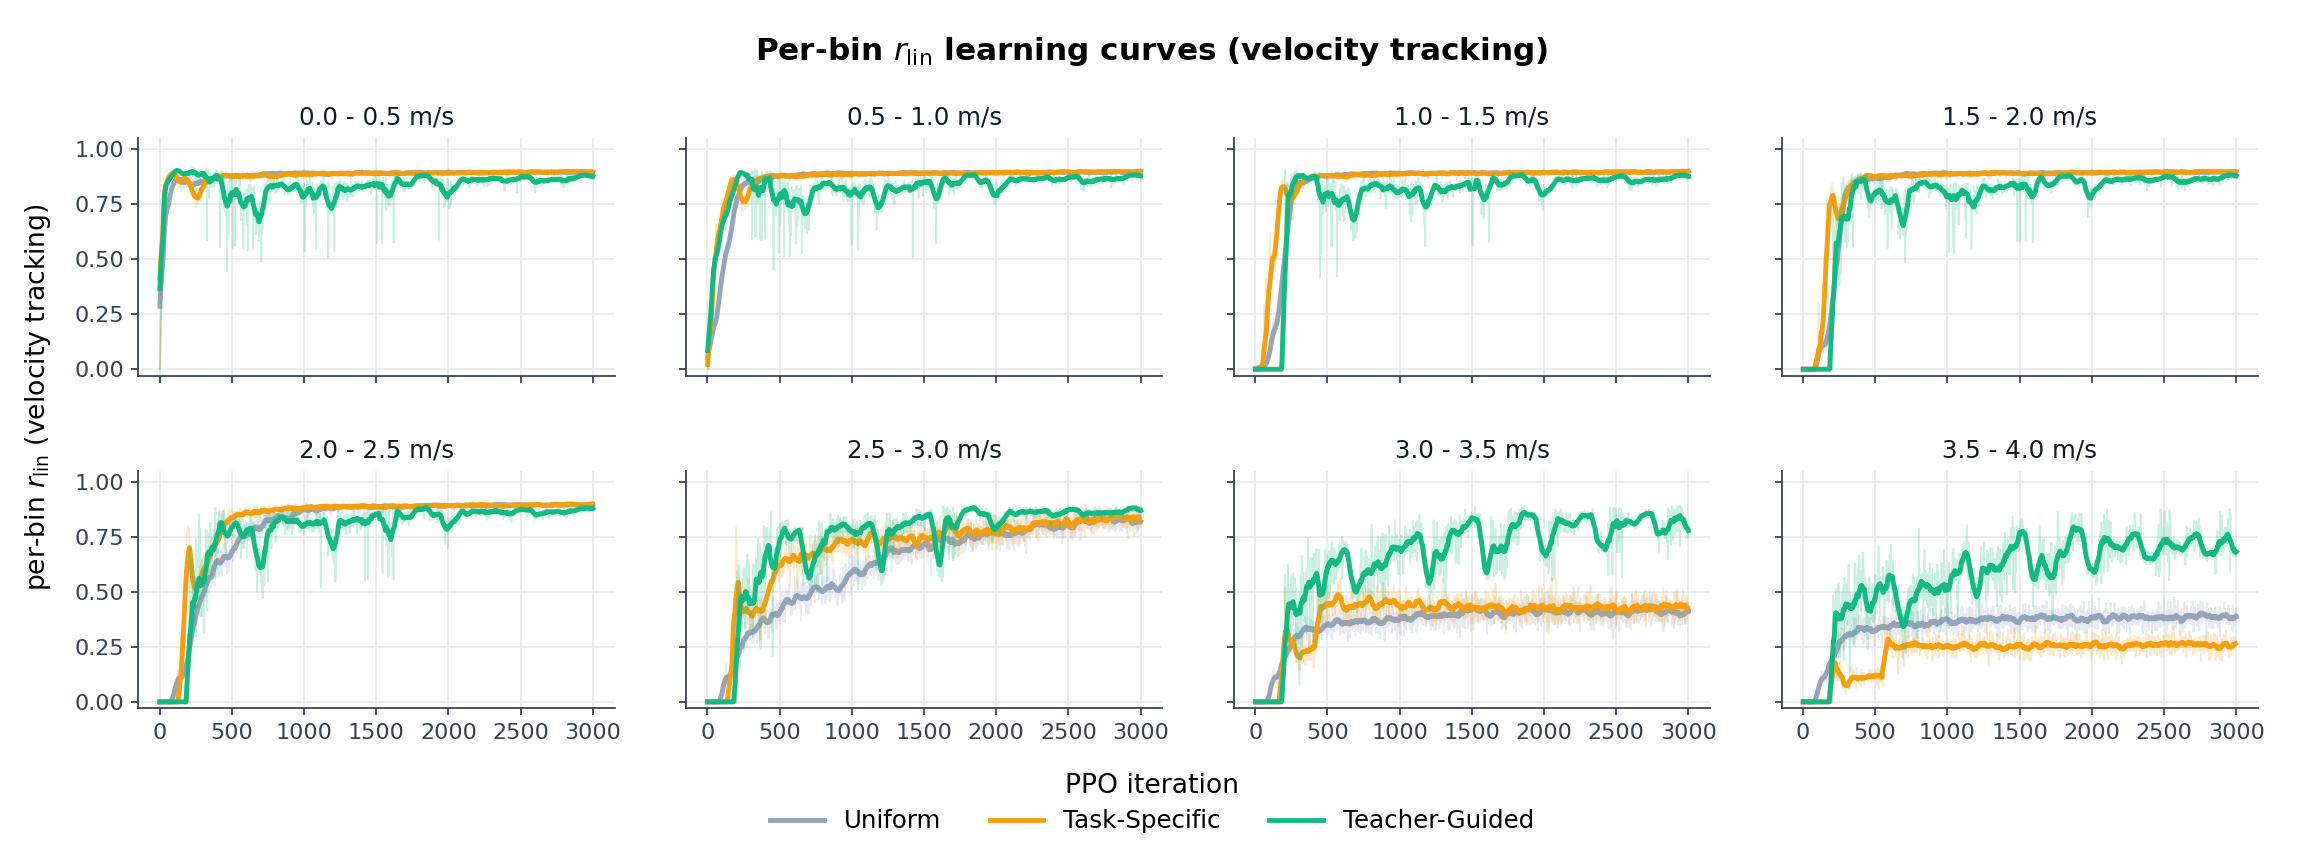
\includegraphics[width=\linewidth]{src/results_phase1_rerun/figures/learning_curves_rlin.png}
\caption{Per-bin tracking reward $R_j$ over training, sprint-retune reward. Bands are $\pm 1$ std across three seeds. Bottom-row bins are the ones that separate uniform from the two curriculum-driven conditions.}
\label{fig:phase1_lc}
\end{figure}

The 3000-iteration budget is short relative to standard practice in this literature. Margolis et al.\ (2022) trained at the equivalent of about 12000 iterations on this scale of robot. The slope-at-end of every cell in Table \ref{tab:phase1_rlin} is at most $10^{-5}$ per iteration, including the bin-6 and bin-7 cells of uniform, so the policies have stopped learning at this budget rather than merely being interrupted partway through. The bin-6 and bin-7 failure of uniform is not a standing-still local optimum. The policy never learned how to take a stride at sprint speed, so it cannot step forward when given the command and loses balance instead (cf.\ \S4.1.3). Training and deterministic evaluation use the same environment and reward and differ only in whether the policy's action noise is on. The failure mode is the same under both protocols.

The reason uniform fails at the sprint bins under the \S3.1.4 reward is the design of the reward itself. The sprint-retune reward contains tracking, smoothness, and feet-air-time terms, but no contact-coordination term, no flight-phase term, and no power term. The policy therefore has to discover a stable sprint gait through exploration alone, and stable sprint near $4$ m/s requires a stride frequency and contact pattern that cannot be reached by simply scaling up a walking gait. Discovering it is sample-hungry. Under uniform sampling each of the eight bins gets $1/8$ of the compute, which is not enough attempts at the sprint bins to stumble on a successful trajectory within $3000$ iterations. Under task-specific sampling, the sprint bins are added to the support only after the lower bins cross $\gamma$, and once added are sampled at the same probability as every other active bin. In this sweep that proves sufficient. By the time bins 6 and 7 unlock there are still on the order of $1500$ iterations left, which is enough to bring the per-bin reward across the mastery threshold. Teacher-guided sampling, with the same reward, also clears bins 6 and 7 within budget, with a similar per-bin reward to task-specific but a different time profile in which the operator concentrates samples on bins where learning progress is detectable. The conclusion at this stage is that \textit{both} curricula succeed under the \S3.1.4 reward while uniform does not. \S4.2 patches the reward directly by adding the energy-regularised term of Liang et al.\ (2024), and \S4.3 re-runs the comparison under the patched reward to separate the operator effect from the reward effect.

The iterations-to-mastery metric (first PPO iteration at which the seed-averaged $R_j$ crosses $\gamma = 0.7$) is summarised in Table \ref{tab:phase1_itm}.

\begin{table}[ht]
\centering
\begin{tabularx}{\textwidth}{@{}r r r r r@{}}
\toprule
\textbf{Bin} & $v_x^{\mathrm{cmd}}$ & \textbf{Uniform} & \textbf{Task-specific} & \textbf{Teacher-guided} \\
\midrule
0 & 0.25 & 30    & 20  & 22 \\
1 & 0.75 & 214   & 134 & 200 \\
2 & 1.25 & 280   & 178 & 290 \\
3 & 1.75 & 340   & 234 & 370 \\
4 & 2.25 & 532   & 284 & 474 \\
5 & 2.75 & 1044  & 334 & 576 \\
6 & 3.25 & not mastered (0/3) & 514 (3/3)  & 874 (3/3) \\
7 & 3.75 & not mastered (0/3) & 1136 (3/3) & 1340 (3/3) \\
\bottomrule
\end{tabularx}
\caption{Iterations-to-mastery per (condition, bin) cell, computed as the first PPO iteration at which the seed-averaged $R_j$ crosses $\gamma = 0.7$. The fraction of seeds that reached mastery individually is shown in parentheses where it is below 3/3.}
\label{tab:phase1_itm}
\end{table}

Bins 0 through 5 are mastered by every condition. Task-specific reaches every one of these bins faster than uniform, because once a bin's mastery threshold is crossed, the support has already expanded to include it and the operator focuses sampling on the new edge. Teacher-guided is comparable to uniform on bins 1 through 4 because the LP-ACRL temperature keeps probability mass spread across all bins as long as multiple bins still show positive learning progress, and it pulls ahead on bins 5, 6, and 7 once the lower bins plateau. Task-specific reaches bins 6 and 7 earlier than teacher-guided, at $514$ versus $874$ at bin 6 and $1136$ versus $1340$ at bin 7, but both operators master both sprint bins within the budget. Uniform masters neither.

\begin{figure}[ht]
\centering
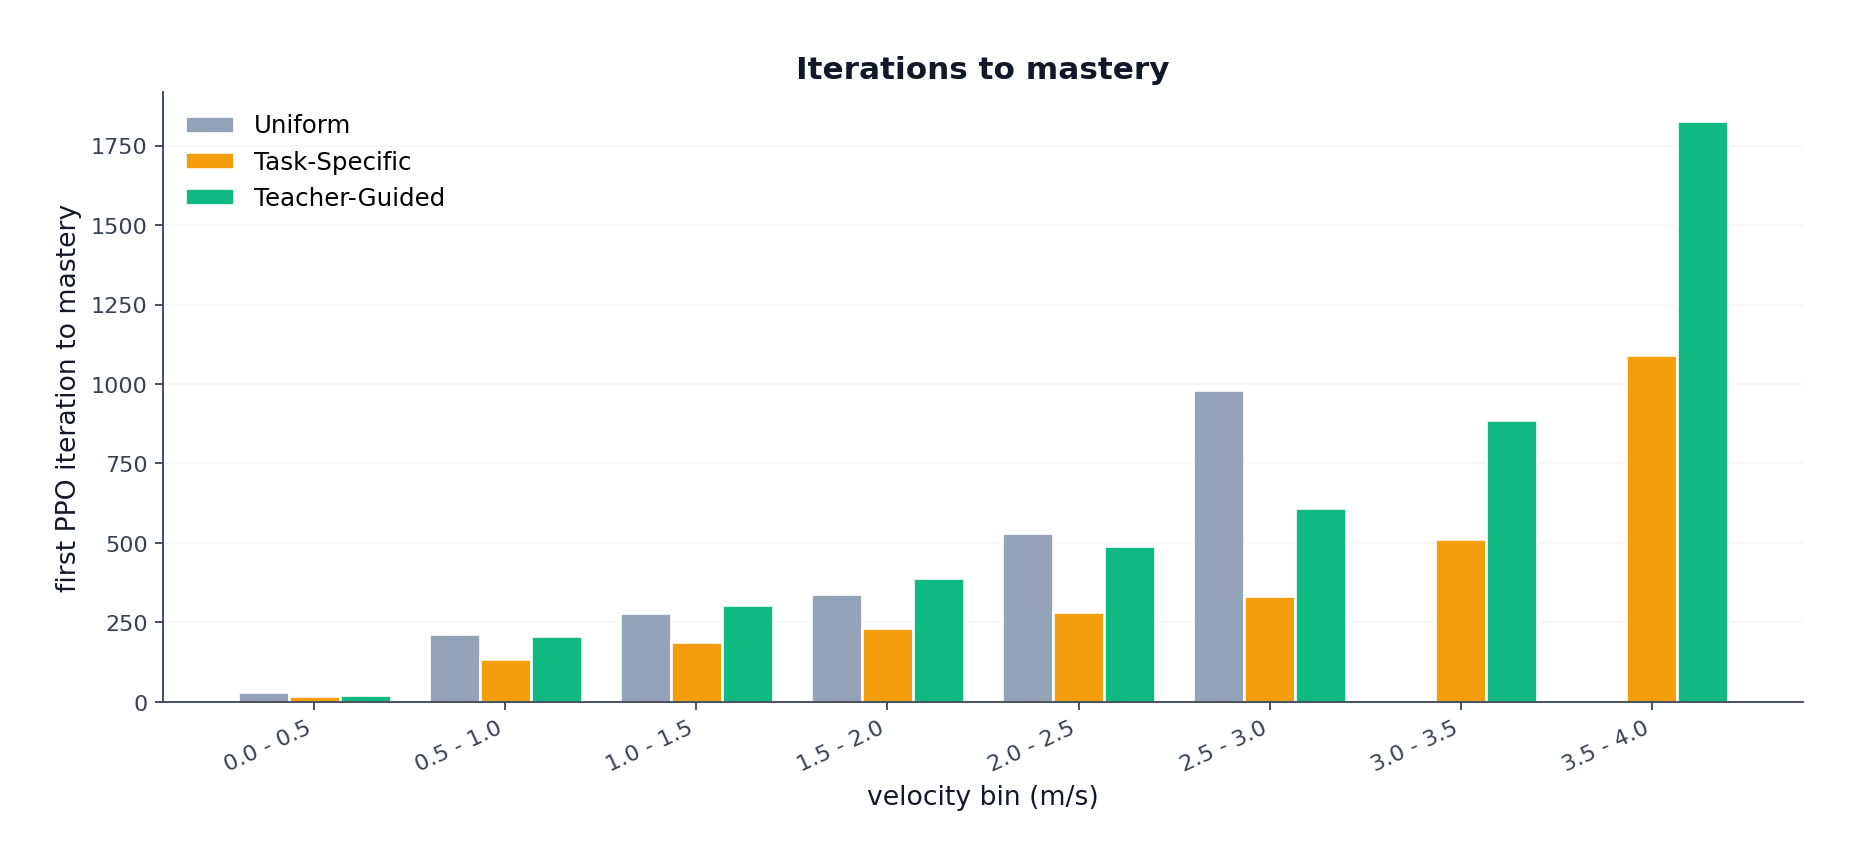
\includegraphics[width=\linewidth]{src/results_phase1_rerun/figures/iterations_to_mastery.png}
\caption{Iterations-to-mastery per (condition, bin), sprint-retune reward. Uniform's bars at bins 6 and 7 are missing because no seed crossed $\gamma$ within the budget.}
\label{fig:phase1_itm}
\end{figure}

Figure \ref{fig:phase1_heatmap} shows the per-bin sampling distribution $c_j(\mathrm{iter})$ as a heatmap. The three rows make the operator behaviour explicit. Uniform is a flat $1/8$ across the eight bins for the full 3000 iterations. Task-specific expands monotonically from bin 0 outward, with every newly-unlocked bin receiving the same probability as the bins below it. Teacher-guided concentrates its mass on the bin with the highest current learning progress, which moves upward across the velocity range as the policy improves at each bin in turn.

\begin{figure}[ht]
\centering
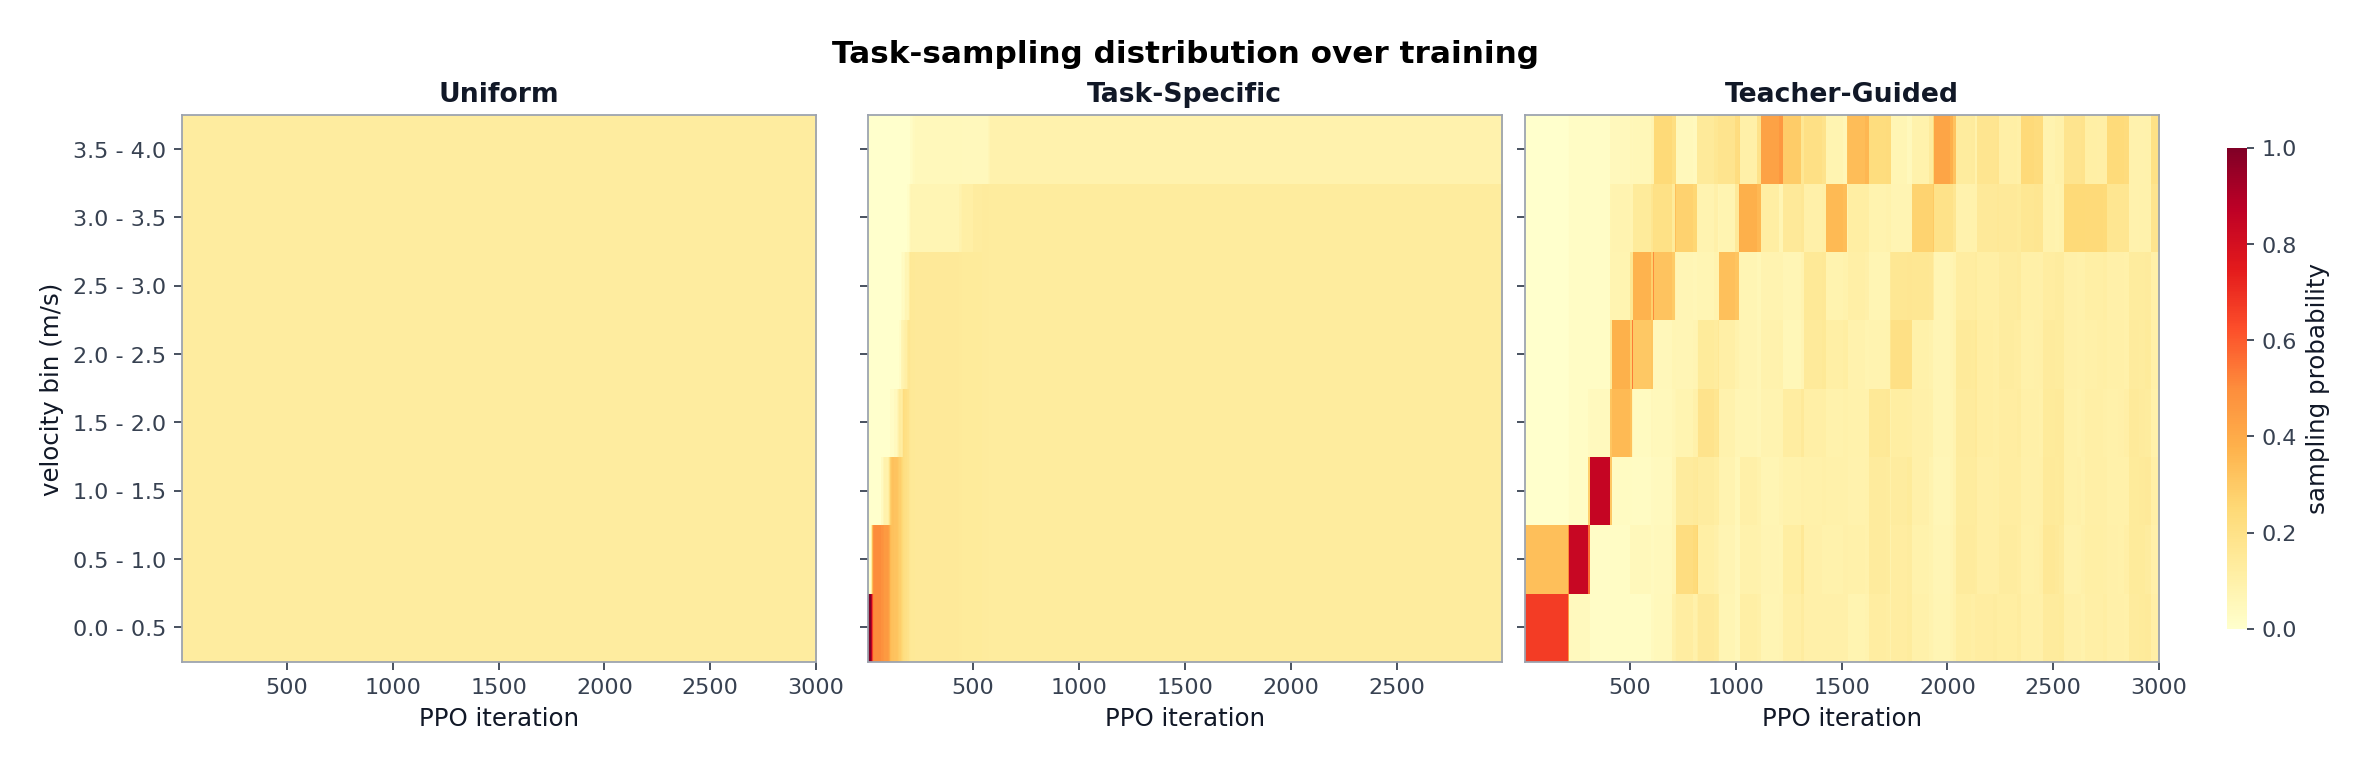
\includegraphics[width=\linewidth]{src/results_phase1_rerun/figures/sampling_heatmap.png}
\caption{Per-bin sampling probability $c_j(\mathrm{iter})$ over training, sprint-retune reward. Bin index on the vertical axis, PPO iteration on the horizontal axis, sampling probability on the colour scale.}
\label{fig:phase1_heatmap}
\end{figure}

\subsubsection{Per-Bin EPTE-SP}

Table \ref{tab:phase1_epte} reports the per-bin EPTE-SP from the deterministic evaluation rollouts of \S3.3, together with the fraction of rollouts that terminated early by falling. EPTE-SP is bounded above at $1.0$ by construction. An EPTE-SP of $1.0$ together with a $100\%$ fall fraction indicates that the deterministic policy is not able to take a single survivable step under that command.

\begin{table}[ht]
\centering
\begin{tabularx}{\textwidth}{@{}r r r r r@{}}
\toprule
\textbf{Bin} & $v_x^{\mathrm{cmd}}$ & \textbf{Uniform EPTE / fall\%} & \textbf{Task-spec EPTE / fall\%} & \textbf{Teacher EPTE / fall\%} \\
\midrule
0 & 0.25 & $0.423$ / $0\%$  & $0.421$ / $1\%$  & $0.368$ / $2\%$ \\
1 & 0.75 & $0.113$ / $0\%$  & $0.103$ / $0\%$  & $0.082$ / $0\%$ \\
2 & 1.25 & $0.074$ / $0\%$  & $0.074$ / $0\%$  & $0.052$ / $0\%$ \\
3 & 1.75 & $0.061$ / $0\%$  & $0.062$ / $0\%$  & $0.052$ / $0\%$ \\
4 & 2.25 & $0.068$ / $0\%$  & $0.070$ / $0\%$  & $0.064$ / $0\%$ \\
5 & 2.75 & $0.151$ / $9\%$  & $0.067$ / $0\%$  & $0.066$ / $0\%$ \\
6 & 3.25 & $0.977$ / $98\%$ & $0.537$ / $50\%$ & $0.187$ / $13\%$ \\
7 & 3.75 & $1.000$ / $100\%$ & $0.536$ / $50\%$ & $0.228$ / $17\%$ \\
\bottomrule
\end{tabularx}
\caption{Per-bin EPTE-SP and fall fraction at deterministic evaluation, averaged across three seeds and 300 rollouts per cell, sprint-retune reward.}
\label{tab:phase1_epte}
\end{table}

The story across bins 0 through 5 is consistent with Table \ref{tab:phase1_rlin}. All three conditions track the command with single-digit-percent error and essentially no falls. The small $9\%$ fall fraction for uniform at bin 5 reflects the policy already wobbling at $2.5$ to $3.0$ m/s. The bin-0 EPTE-SP values are high in absolute terms at about $0.4$ because EPTE-SP is normalised by command magnitude, and a $0.1$ m/s tracking error at the $0.25$ m/s bin centre divides into a $40\%$ percentage error. This is an artifact of the normalisation rather than a control failure, since the mean measured forward velocity at bin 0 is between $0.18$ and $0.19$ m/s across all three conditions.

The collapse at bins 6 and 7 mirrors the training-time tracking-reward separation but is \textit{finer-grained} than it. Under deterministic evaluation, task-specific is intermediate rather than lumped with uniform. Uniform falls $98\%$ at bin 6 and $100\%$ at bin 7. Task-specific falls $50\%$ at both sprint bins, and teacher-guided falls $13\%$ at bin 6 and $17\%$ at bin 7. EPTE-SP mirrors the same ranking. Two factors separate task-specific from teacher-guided here despite their similar training-time $R_j$ on bins 6 and 7. First, teacher-guided invested more total samples on each sprint bin once it reached them, so the underlying policy is more robust. Second, under deterministic evaluation the action noise is removed, and a policy that succeeded stochastically by sometimes-lucky strides regresses more than one that converged tightly.

\begin{figure}[ht]
\centering
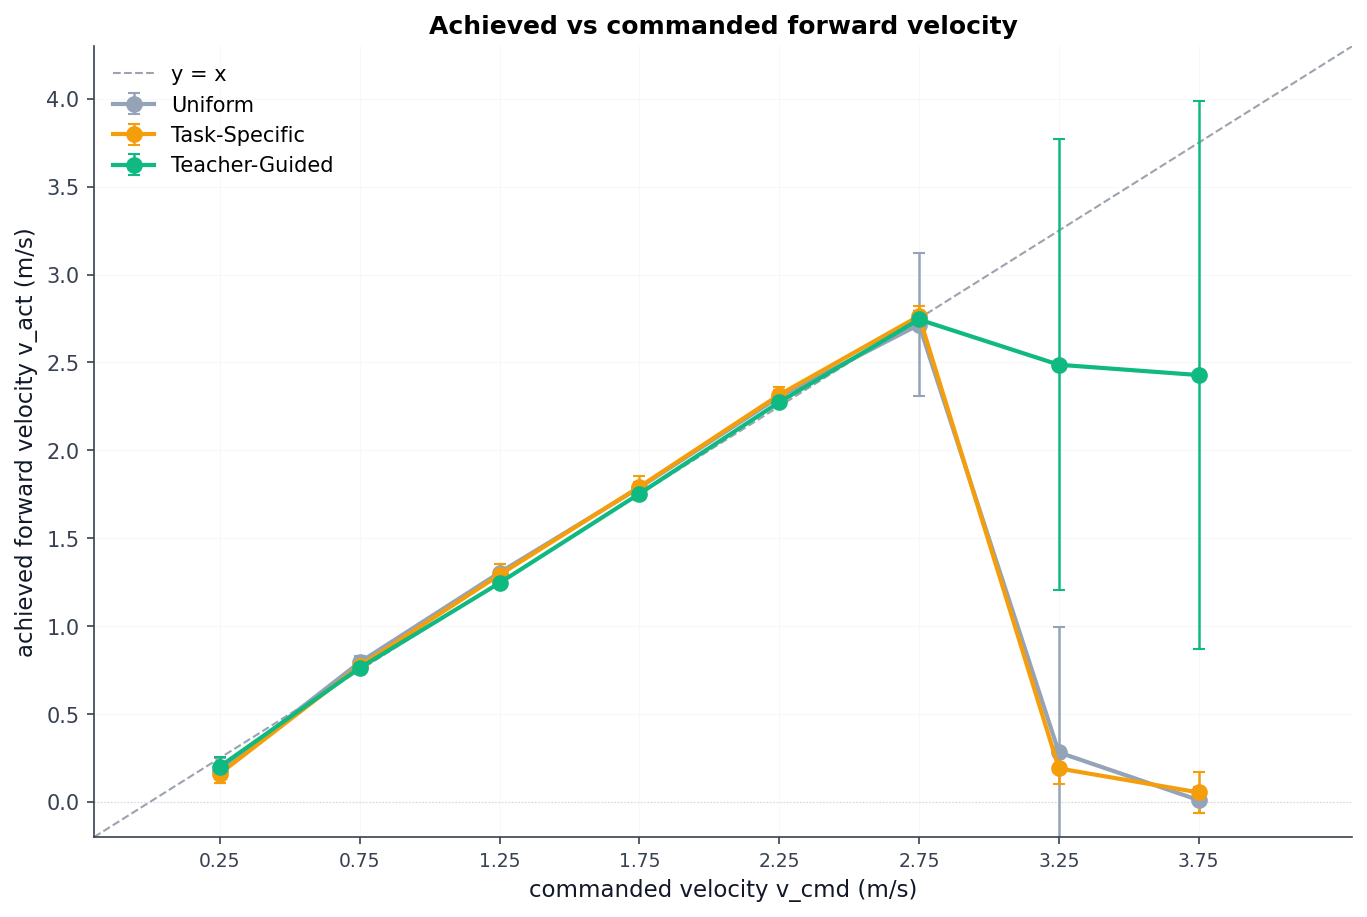
\includegraphics[width=\linewidth]{src/results_phase1_rerun/figures/v_actual_vs_cmd.png}
\caption{Mean measured forward velocity vs commanded velocity, sprint-retune reward. Diagonal is the perfect-tracking reference. Uniform's points at bins 6 and 7 sit near $\bar v_x = 0$; task-specific reaches roughly half-speed at the sprint bins; teacher-guided is the closest to the diagonal at bins 6 and 7.}
\label{fig:phase1_vvscmd}
\end{figure}

Figure \ref{fig:phase1_vvscmd} plots the per-bin mean forward velocity at evaluation against the command. At bins 6 and 7, uniform stops at $0.21$ m/s and $0.08$ m/s against commands of $3.25$ and $3.75$ m/s. Task-specific reaches $1.73$ m/s and $1.81$ m/s in the same bins, roughly half the commanded sprint speed, which is a real running gait that survives half the deterministic rollouts. Teacher-guided reaches $2.85$ m/s and $2.97$ m/s in the same bins, closer to but still below the commanded velocity, and falls in only about $15\%$ of rollouts. The EPTE-SP rank at bins 6 and 7 in which uniform is much larger than task-specific which is in turn larger than teacher-guided is therefore driven by both how fast the policy tracks the command and how often it survives the rollout.

\begin{figure}[ht]
\centering
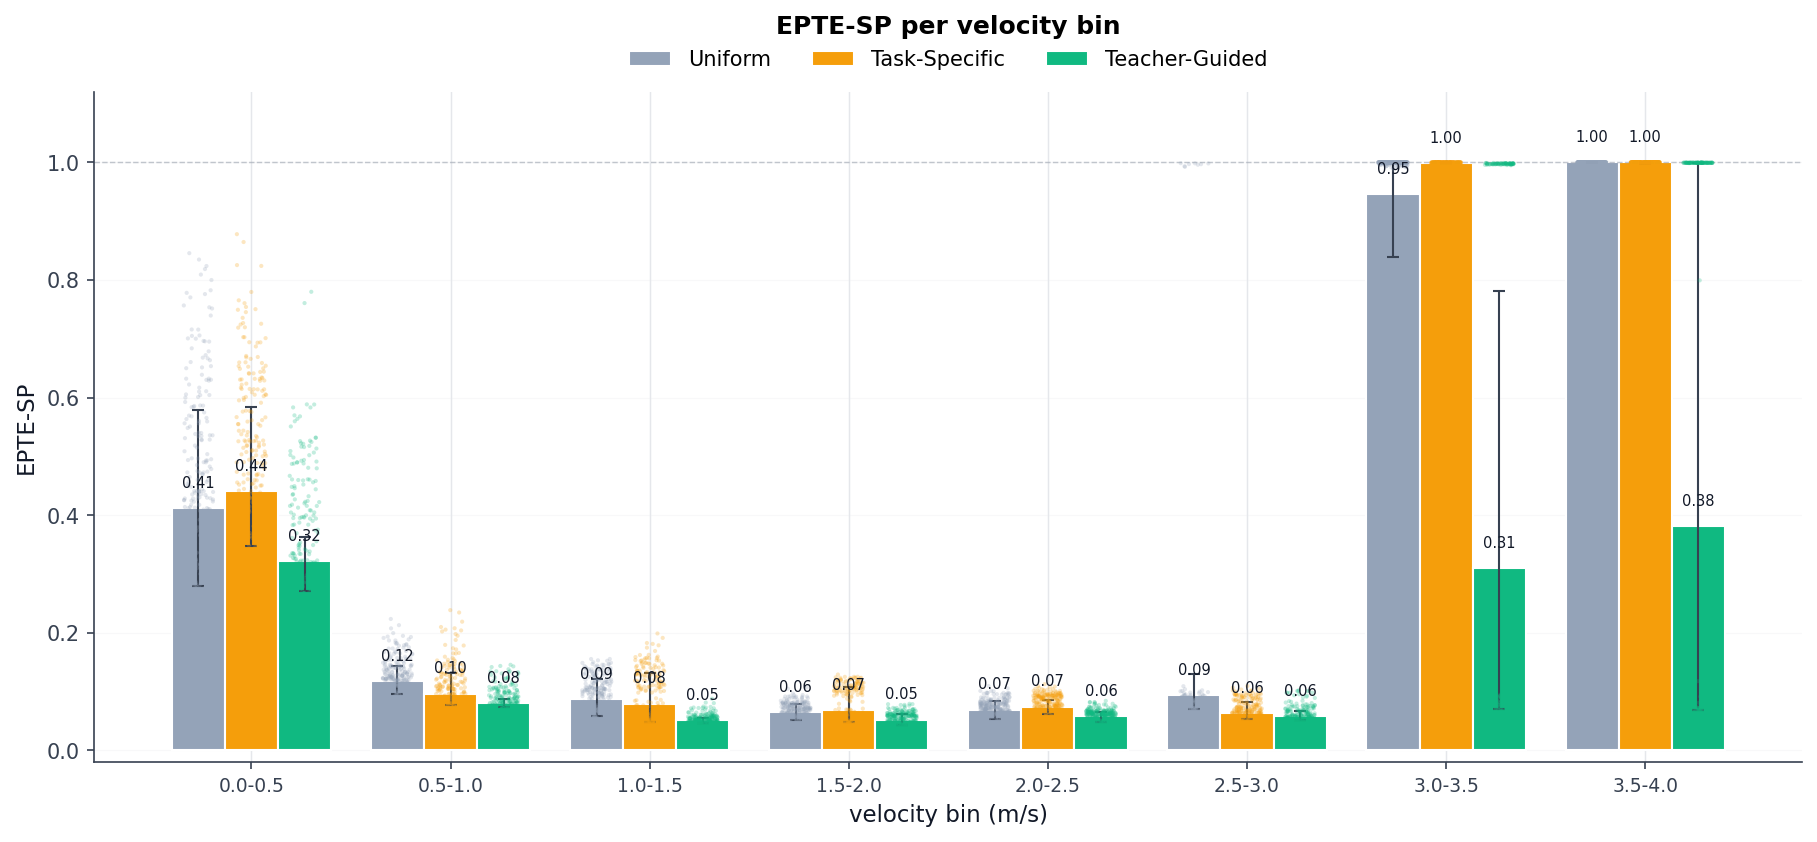
\includegraphics[width=\linewidth]{src/results_phase1_rerun/figures/epte_bars.png}
\caption{EPTE-SP per (condition, bin), sprint-retune reward. The saturated bar at bin 7 of uniform corresponds to the $100\%$-fall column of Table \ref{tab:phase1_epte}; task-specific's bin-6 and bin-7 bars at $\sim 0.54$ reflect its $50\%$ fall fraction at the sprint bins.}
\label{fig:phase1_epte}
\end{figure}

\subsubsection{Qualitative Behaviour at Evaluation}

The visual signature of the sprint-retune reward depends on which bin is being evaluated. Two qualitatively different failure modes appear at the extremes of the velocity range and are visible in Figure \ref{fig:phase1_gait}.

\begin{figure}[ht]
\centering
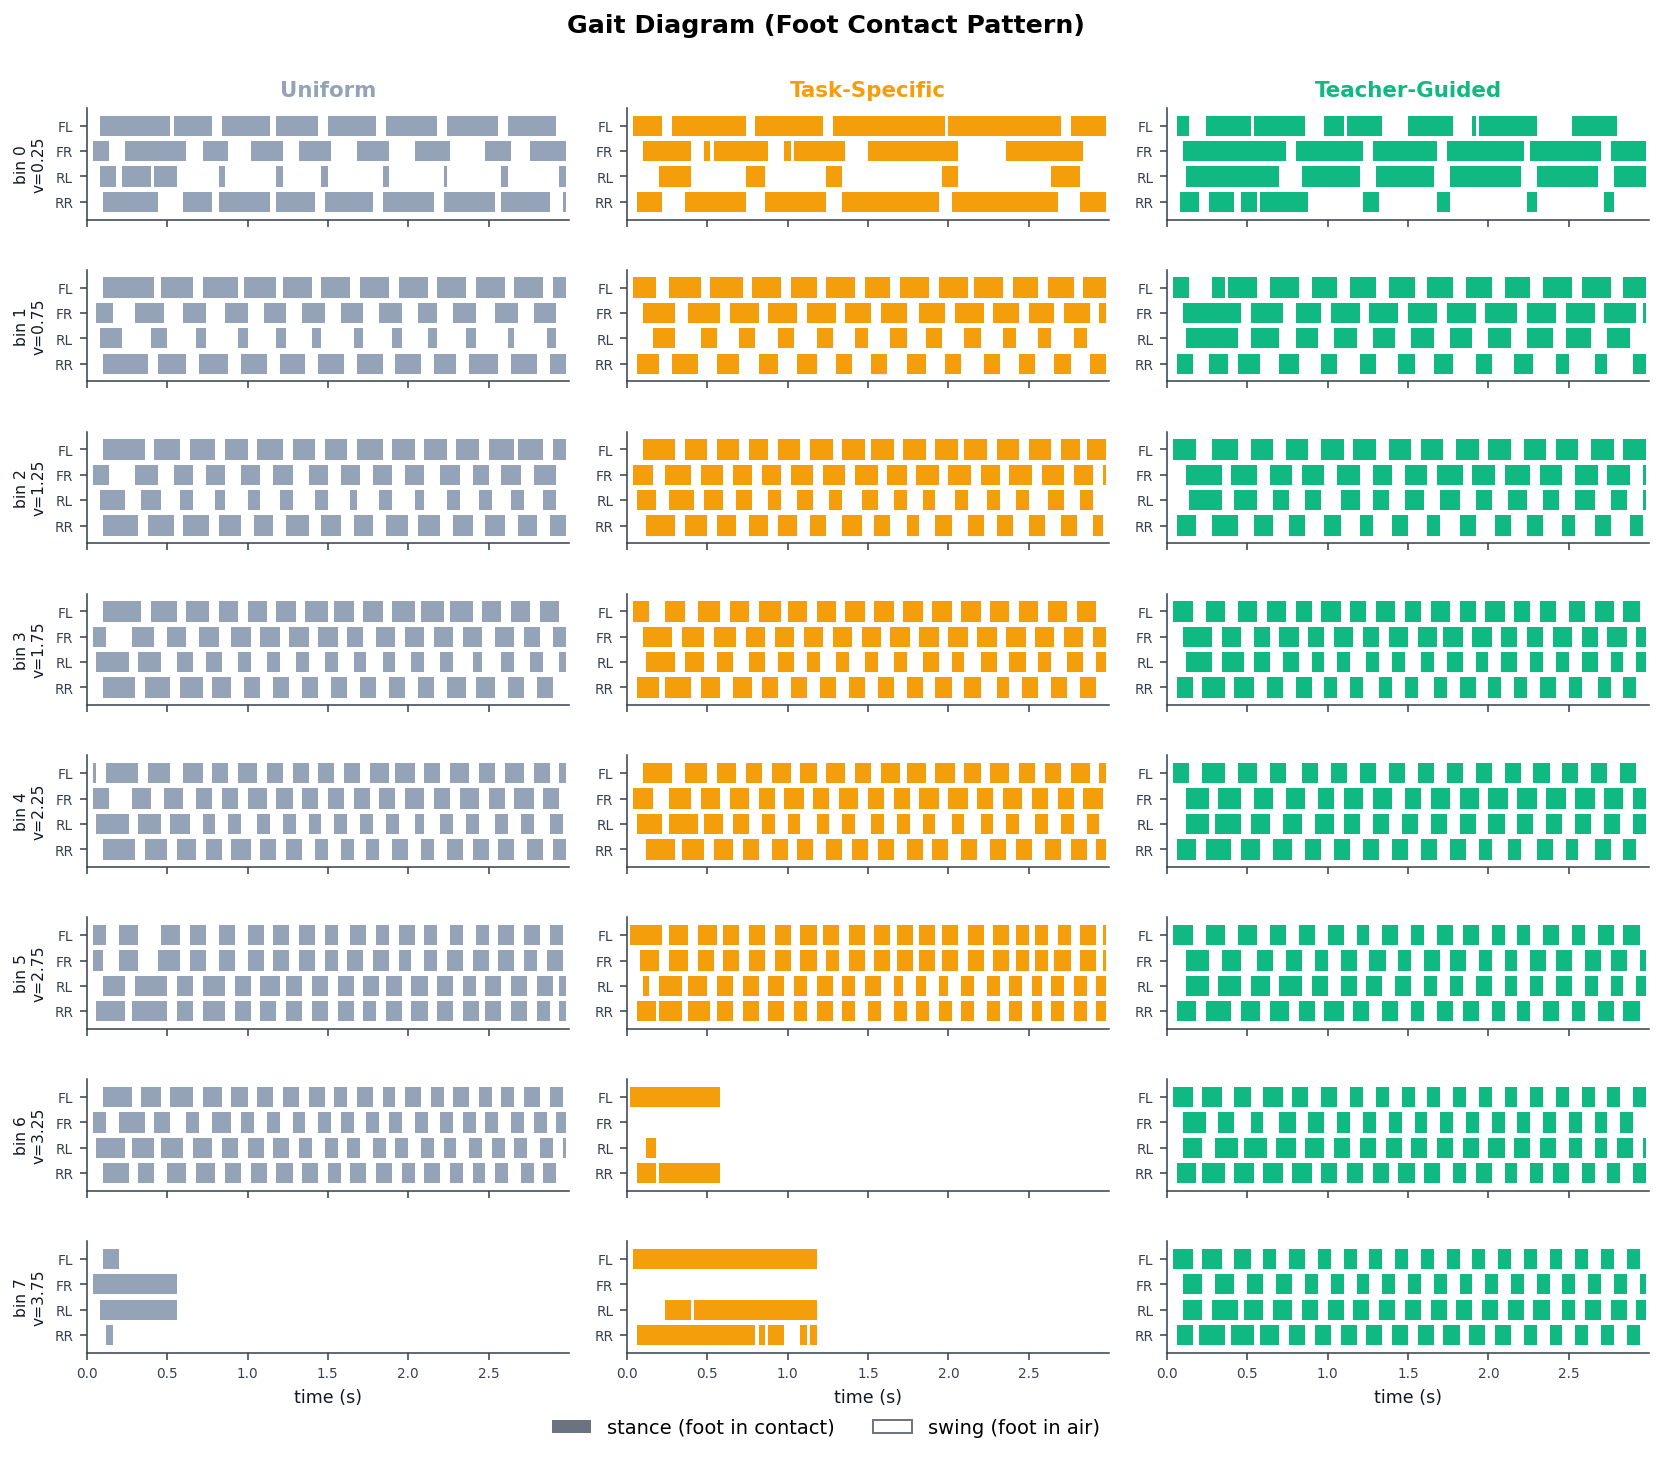
\includegraphics[width=\linewidth]{src/results_phase1_rerun/figures/gait_diagram.png}
\caption{Gait diagram at deterministic evaluation, sprint-retune reward. Columns are conditions (uniform / task-specific / teacher-guided), rows are velocity bins. Coloured blocks mark stance (foot in contact); white gaps mark swing. Per cell the plotted rollout is the best-surviving rollout across the three seeds, with ties broken by closest mean forward velocity to the command.}
\label{fig:phase1_gait}
\end{figure}

\textbf{Low bins. Irregular contact at slow command speed.} At a commanded velocity of $0.25$ m/s the Phase 1 gait classifier labels all three conditions as \textit{Irregular} in Figure \ref{fig:phase1_gait}. The per-foot contact pattern does not match any canonical walk template, and the duty factor and stride frequency reported in \S4.3.3 for the same bin under the energy-regularised reward are absent here because no consistent stride cycle is being produced. The policy nevertheless meets the slow commanded forward velocity at about $0.19$ m/s against the $0.25$ m/s command, and the chassis stays upright with a fall fraction below $2\%$ across the three conditions in Table \ref{tab:phase1_epte}. The qualitative outcome is that the policy never learned a real walking gait at the slow command. The command is slow enough that any non-falling foot motion satisfies the tracking term $r_{\mathrm{lin}}$, and the \S3.1.4 reward contains no term that would penalise the absence of a canonical gait pattern, so the policy settles in an irregular contact pattern that scores well without learning to walk properly.

\textbf{High bins. Failure to learn under uniform.} At $v_x^{\mathrm{cmd}} \ge 3.0$ m/s under uniform, Figure \ref{fig:phase1_gait} shows the rollout terminating early. The bin-6 and bin-7 cells in the uniform column are short stance/swing fragments that end before a full stride completes. The policy never learned how to step forward at sprint speed, so it cannot move at the commanded velocity and loses balance before the rollout ends (cf.\ the $98$--$100\%$ fall column of Table \ref{tab:phase1_epte}). This is not a reward hack. It is a learning failure within the $3000$-iteration budget at these bins. The task-specific and teacher-guided columns at the same bins show all four feet cycling through stance and swing for the full evaluation window in a Trot (walking) pattern (duty $\beta \approx 0.52$--$0.54$, diagonal pair near-synchronous), so the high-bin failure is specific to the operator that under-samples the sprint bins, not to the reward.

\textbf{Why the \S3.1.4 reward allows the low-bin failure.} The tracking term $r_{\mathrm{lin}}$ scores forward velocity indifferent to how that velocity is generated. The feet-air-time bonus with threshold $0.1$ s in Table \ref{tab:sprint_retune} is the only term in \S3.1.4 designed to shape the contact pattern, and it scores each foot independently. Nothing in the reward depends on the coordination \textit{between} feet. An irregular four-foot contact pattern therefore scores just as well as a clean canonical walk as long as the body drifts forward at the slow commanded speed, and the policy lands on whichever contact pattern is gradient-cheapest to reach. The same absence of contact-coordination is the reason uniform never escapes the high-bin failure either. The reward gives no gradient signal for \textit{which} contact structure to use at sprint, so the only way for the operator to find a sprint gait that actually steps forward is to stumble on it by exploration, and uniform does not do this within $3000$ iterations at the $1/8$ sampling share each sprint bin receives.

\textbf{Deployment implication.} The project goal is a single PPO policy that tracks forward-velocity commands across $[0,\,4]$ m/s. The sprint-retune reward partially fails this goal in two different ways. Every condition produces an irregular contact pattern at the low bin, and uniform cannot step forward at the sprint bins at all. Task-specific and teacher-guided both reach the sprint bins under this reward, but they still produce the low-bin irregularity, so the curriculum alone does not rescue the low-bin failure. A different reward shape is needed. \S4.2 introduces one in which the contact coordination between feet enters the reward through an energy-cost-of-transport term.

\subsection{From Sprint-Retune to Energy Regularisation}

The reward term added to fix the \S4.1.3 observation has to depend on the relative timing of foot contacts. Liang et al.\ (2024) report that a single energy-regularised term, added to a tracking objective, causes the policy to autonomously transition between walking, trotting, and fly-trotting as the command rises, without any contact-phase reference being supplied during training. The term depends on contact timing indirectly through its cost-of-transport interpretation. It penalises mechanical power normalised by command magnitude. The four-foot bound carries a higher power cost per unit of forward motion than an alternating gait does, so under the energy term the alternating pattern scores higher. This project adopts Liang's approach because it requires no hand-coded gait template and because the existing \S3.1.4 reward already supplies the tracking block that the Liang reward composes with. Liang's claim is empirical, so the same gait family has to be verified on the Go2. That verification is \S4.3.4.

The remainder of this section reproduces the Liang reward in its source notation (\S4.2.1) and explains the procedure used to fix its scale parameters on the Go2 (\S4.2.2). The matched three-condition comparison under the calibrated reward is reported in \S4.3.

\subsubsection{The Liang Energy-Regularised Reward}

Liang et al.\ (2024) consider a single PPO policy on the Unitree Go1 quadruped tracking forward-velocity and yaw-rate commands. The total per-step reward is written as a multiplicative composition of three blocks,

\[
R = (R_{\mathrm{motion}} + R_{\mathrm{energy}}) \cdot f(R_{\mathrm{aux}}), \tag{1}
\]

where $R_{\mathrm{motion}}$ scores command tracking, $R_{\mathrm{energy}}$ scores energetic efficiency, and $f(R_{\mathrm{aux}})$ is a positive multiplicative wrapping of an auxiliary term $R_{\mathrm{aux}}$ that aggregates the smoothness and safety penalties.

The specific choice of $f$ in the paper is the exponential, so that the auxiliary block acts as a unit-bounded multiplier on the motion-plus-energy sum,

\[
R = \big( R_{\mathrm{motion}} + \alpha_{\mathrm{en}}\, R_{\mathrm{en}}(v_x, \omega_z) \big) \cdot \exp\!\big( - R_{\mathrm{aux}} \big), \tag{2}
\]

where $\alpha_{\mathrm{en}} \ge 0$ is the scalar weight on the energy block.

The motion block decomposes into a linear-velocity term and an angular-velocity term,

\[
R_{\mathrm{motion}} = R_{\mathrm{lin}} + \alpha_{\mathrm{ang}}\, R_{\mathrm{ang}},
\]

\[
R_{\mathrm{lin}} = \exp\!\left( - \frac{ |v_x - \hat v_x|^2 + |v_y - \hat v_y|^2 }{\sigma_v} \right),
\]

\[
R_{\mathrm{ang}} = \exp\!\left( - \frac{ |\omega_z - \hat\omega_z|^2 }{\sigma_\omega} \right), \tag{3}
\]

where $\hat v_x, \hat v_y$ are the commanded linear-velocity components, $\hat\omega_z$ is the commanded yaw rate, $v_x, v_y, \omega_z$ are the measured values, and $\sigma_v, \sigma_\omega$ are scale parameters that control the width of the tracking kernel.

The energy block is the new ingredient. Liang et al.\ (2024) define it as

\[
R_{\mathrm{en}} = \exp\!\left( - \frac{ \sum_i \, |\tau_i| \, |\dot q_i| }{ \sigma_{\mathrm{en},x}\, |v_x| + \sigma_{\mathrm{en},z}\, |\omega_z| } \right), \tag{4}
\]

where $\tau_i$ is the applied joint torque on actuator $i$, $\dot q_i$ is the corresponding joint velocity, the sum runs over all actuated joints, and $\sigma_{\mathrm{en},x},\, \sigma_{\mathrm{en},z}$ are scale parameters that set the cost-of-transport scale on linear and angular motion respectively.

Three design choices in (4) are non-obvious and they each have a behavioural consequence.

\begin{itemize}
  \item \textbf{Absolute values inside the sum.} The numerator uses $|\tau_i|\,|\dot q_i|$ rather than the signed product $\tau_i \dot q_i$. The signed product would be the net mechanical power flowing out of the actuator, which can be negative when the joint is braking. The absolute-value form charges the policy for braking energy as if it were positive energy expenditure, on the grounds that the physical motor does not regenerate that energy back into the battery. This is what the paper means by treating $\sum_i |\tau_i||\dot q_i|$ as a proxy for instantaneous power draw rather than as net mechanical work.
  \item \textbf{Denominator as a command-magnitude scale.} The denominator $\sigma_{\mathrm{en},x}|v_x| + \sigma_{\mathrm{en},z}|\omega_z|$ is proportional to the measured speed of motion. The ratio inside the exponential is therefore (power) / (speed-scale), which has units of force times a per-axis scale, i.e.\ a cost of transport. The implication is that the same power draw is penalised less harshly when the robot is moving fast than when it is moving slow. The reward is shaped around energy \textit{per unit of useful motion}, not energy per unit of time.
  \item \textbf{Exponential wrapping.} The exponential makes $R_{\mathrm{en}} \in (0, 1]$, so it integrates additively into the motion block of (2) without dominating the tracking reward at any one timestep. There is no separate contact-schedule reward. The only thing pushing the policy toward an alternating gait is the cost-of-transport interpretation of the denominator.
\end{itemize}

The reported defaults for the Go1 are $\sigma_{\mathrm{en},x} = 1000$, $\sigma_{\mathrm{en},z} = 500$, $\alpha_{\mathrm{en}} = 1.0$, and $\sigma_v = \sigma_\omega = 0.25$, on the forward-velocity range $v_x \in [0,\, 2.5]$ m/s. Liang et al.\ report an ablation in which setting $\alpha_{\mathrm{en}} = 0$ (energy block disabled) yields the bouncing four-foot synchronised gait described above, while $\alpha_{\mathrm{en}} = 1.0$ yields a walking pattern at low command speed, a two-beat trot at moderate command speed, and a fly-trotting pattern with a flight phase at high command speed, with no contact reference supplied at any point during training.

This project's energy-regularised reward configuration uses (4) as written, with $\sigma_{\mathrm{en},x}$, $\sigma_{\mathrm{en},z}$, $\alpha_{\mathrm{en}}$, and $\sigma_v$ fixed by the calibration of \S4.2.2 and a small clamping $\max(\cdot,\,\varepsilon)$ added to the denominator of (4) to bound the gradient at very low commanded speed.

\subsubsection{Calibrating the Energy Scale}

The reward of (4) has one knob that matters. That knob is $\sigma_{\mathrm{en},x}$, the linear-speed entry in the denominator, with $\sigma_{\mathrm{en},z} = 0.5\,\sigma_{\mathrm{en},x}$ fixed by the ratio Liang et al.\ (2024) used. The behaviour of $R_{\mathrm{en}} = \exp(-x)$ depends on where this knob places the argument $x$. If $\sigma_{\mathrm{en},x}$ is too small, $x$ is large and $R_{\mathrm{en}}$ collapses near zero. The energy term then swamps the tracking term and the policy stops tracking. If $\sigma_{\mathrm{en},x}$ is too large, $x$ is small and $R_{\mathrm{en}}$ saturates near one. The energy term is then a near-constant offset on the policy gradient and the policy ignores it. Only a middle $\sigma_{\mathrm{en},x}$ gives the policy a usable gradient from $R_{\mathrm{en}}$.

Liang et al.\ (2024) report $\sigma_{\mathrm{en},x} = 1000$ for the Unitree Go1 on $v_x \in [0,\, 2.5]$ m/s. This project uses a different robot (Go2) and a wider command range ($v_x \in [0,\, 4]$ m/s). The joint-power numerator and the command-magnitude denominator of $R_{\mathrm{en}}$ both depend on the robot and the range, so Liang's value is not guaranteed to fall in the middle regime on the Go2. The right $\sigma_{\mathrm{en},x}$ has to be found by calibration.

The calibration is split into two cheap stages.

\textbf{Step 1, no training. Find which $\sigma_{\mathrm{en},x}$ values keep the gradient alive at all.} Run the Go2 in Isaac Lab for a fixed number of steps under a uniformly-random joint-action policy. The robot will twitch in place without making real forward motion. At each step record the joint power proxy $P = \sum_i |\tau_i|\,|\dot q_i|$, the forward speed $|v_x|$, and the yaw rate $|\omega_z|$. Plug each candidate $\sigma_{\mathrm{en},x}$ from a logarithmic grid into the $R_{\mathrm{en}}$ formula, compute the mean of $R_{\mathrm{en}}$ across the rollout, and keep only the $\sigma_{\mathrm{en},x}$ values for which this mean lies in $[0.3,\, 0.75]$. That range is the steep middle region of the exponential. Values of $\sigma_{\mathrm{en},x}$ that produce a mean below it have already saturated $R_{\mathrm{en}}$ near zero, so the energy term would swamp tracking. Values above it have saturated near one, so the energy term acts as a constant offset that the policy ignores.

The reason random actions are used as the test signal is that they are the worst case the policy will ever see. Power draw is high and forward motion is near zero, so $x$ is at its largest and $R_{\mathrm{en}}$ at its smallest. A $\sigma_{\mathrm{en},x}$ that lands the random-action mean inside the steep region is guaranteed to keep $R_{\mathrm{en}}$ in or above the steep region for the entire rest of training, because every improvement in the policy reduces $x$ and pushes $R_{\mathrm{en}}$ upward. The energy term gently fades out as the gait improves, which is the desired behaviour.

There are three things Step 1 cannot do. It cannot tell us how the energy block should be weighted against the tracking block (the parameter $\alpha_{\mathrm{en}}$ in equation 2). It cannot tell us how strict the tracking kernel should be (the parameter $\sigma_v$). And it cannot verify that the live PPO gradient actually drives the policy to a walking or trotting gait once training starts. All three gaps are closed by a small training experiment.

\textbf{Step 2, short training. Pick the configuration with the best tracking and a meaningful gait differential.} Take three $\sigma_{\mathrm{en},x}$ values from the Step 1 bracket (one near the low edge, one in the middle, one near the high edge) and combine them with three choices of $(\sigma_v,\,\alpha_{\mathrm{en}})$. The result is a $3 \times 3$ grid of nine combinations. For each combination, train a single uniform-sampling policy under the energy-regularised reward for a reduced number of iterations. After training, run each of the nine policies through the standard \S3.3 evaluation on all eight velocity bins and record two scalars per run. The first scalar is the sum of per-bin tracking error across the eight bins. The second is the duty-factor differential $\beta_{b_0} - \beta_{b_4}$ between the slowest and the middle bin. The cell with the lowest summed tracking error, subject to a non-degenerate duty differential, is the one whose $(\sigma_{\mathrm{en},x},\,\sigma_{\mathrm{en},z},\,\sigma_v,\,\alpha_{\mathrm{en}})$ tuple is frozen and reused unchanged for the matched three-condition sweep of \S4.3.

In one sentence: Step 1 throws away the $\sigma_{\mathrm{en},x}$ values where the reward gradient is dead before training even starts, and Step 2 trains the survivors and keeps the one with the best tracking error across the eight bins.

\textbf{Step 1 result.} Table \ref{tab:step1} reports the Step 1 random-action diagnostic for seven candidate $\sigma_{\mathrm{en},x}$ values on a logarithmic grid. The mean instantaneous power proxy was $100.2$ W, the mean $|v_x|$ was $0.10$ m/s, and the mean $|\omega_z|$ was $0.35$ rad/s.

\begin{table}[ht]
\centering
\begin{tabularx}{\textwidth}{@{}r r r X@{}}
\toprule
$\sigma_{\mathrm{en},x}$ & mean $R_{\mathrm{en}}$ & std $R_{\mathrm{en}}$ & regime \\
\midrule
$50$   & $0.013$ & $0.046$ & too strong (saturated near $0$) \\
$100$  & $0.063$ & $0.097$ & strong \\
$250$  & $0.240$ & $0.191$ & strong \\
$500$  & $0.436$ & $0.223$ & useful gradient \\
$1000$ & $0.627$ & $0.207$ & useful gradient \\
$2000$ & $0.775$ & $0.163$ & weak gradient \\
$5000$ & $0.895$ & $0.099$ & weak gradient \\
\bottomrule
\end{tabularx}
\caption{Step 1 random-action diagnostic on the Go2 under the \S3 simulation configuration, $1000$ random-action steps per candidate $\sigma_{\mathrm{en},x}$. Values inside the $[0.3,\,0.75]$ band are those for which $R_{\mathrm{en}}$ is in the steep region of its argument; values outside the band give a flat gradient.}
\label{tab:step1}
\end{table}

\begin{figure}[ht]
\centering
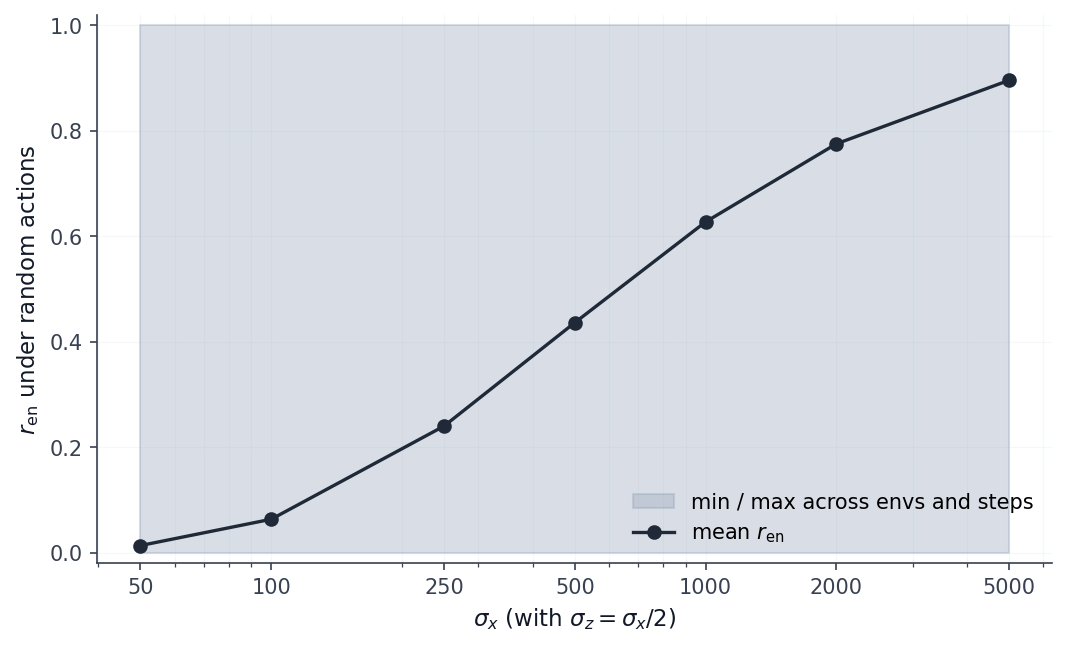
\includegraphics[width=\linewidth]{src/results_phase2_rerun/figures/sigma_phase0.png}
\caption{Step 1 random-action diagnostic. Mean $R_{\mathrm{en}}$ across the rollout (dark line) and per-environment min/max envelope (grey band) as a function of $\sigma_{\mathrm{en},x}$ on the logarithmic grid of Table \ref{tab:step1}.}
\label{fig:step1}
\end{figure}

Only $\sigma_{\mathrm{en},x} \in \{500, 1000\}$ fall inside the target band. The value $250$ is just below at $0.240$ and $2000$ is just above at $0.775$. The Step 2 grid is anchored on the in-band pair and reaches into the just-below band to verify that the calibration does not lose tracking quality at the low end. The three $\sigma_{\mathrm{en},x}$ values selected for the grid are $\{500,\, 750,\, 1000\}$, and they are crossed with $(\sigma_v,\,\alpha_{\mathrm{en}}) \in \{(0.5, 1.0),\, (1.0, 1.0),\, (1.0, 0.5)\}$.

\textbf{Step 2 result.} Table \ref{tab:step2} reports the $3 \times 3$ calibration grid evaluated under the deterministic protocol of \S3.3. Each grid cell was trained for $1500$ PPO iterations under uniform sampling. The three columns track different aspects of the resulting policy: the summed per-bin tracking error $\sum_j \mathrm{err}_j$ across all eight bins, the duty-factor differential between the lowest and the mid bin ($\beta_{b_0} - \beta_{b_4}$), and the wall-clock cost.

\begin{table}[ht]
\centering
\begin{tabularx}{\textwidth}{@{}r r r r r r r@{}}
\toprule
\textbf{Run} & $\sigma_{\mathrm{en},x}$ & $\sigma_v$ & $\alpha_{\mathrm{en}}$ & $\sum_j$ err & $\beta_{b_0} - \beta_{b_4}$ & wall-clock (min) \\
\midrule
1 & $500$  & $0.5$ & $1.0$ & $2.922$ & $0.155$ & $32.4$ \\
2 & $750$  & $0.5$ & $1.0$ & $2.333$ & $0.088$ & $33.8$ \\
3 & $1000$ & $0.5$ & $1.0$ & $2.487$ & $0.099$ & $32.9$ \\
4 & $500$  & $1.0$ & $1.0$ & $1.787$ & $0.105$ & $36.4$ \\
5 & $750$  & $1.0$ & $1.0$ & $1.750$ & $0.183$ & $34.5$ \\
6 & $1000$ & $1.0$ & $1.0$ & $1.627$ & $0.143$ & $33.7$ \\
\textbf{7} & $\mathbf{500}$ & $\mathbf{1.0}$ & $\mathbf{0.5}$ & $\mathbf{1.537}$ & $\mathbf{0.143}$ & $\mathbf{37.5}$ \\
8 & $750$  & $1.0$ & $0.5$ & $1.798$ & $0.137$ & $38.6$ \\
9 & $1000$ & $1.0$ & $0.5$ & $1.585$ & $0.104$ & $32.0$ \\
\bottomrule
\end{tabularx}
\caption{Step 2 calibration grid. Each row is a separate uniform-sampling training run at $1500$ PPO iterations under the energy-regularised reward. Tracking-quality column is the sum of per-bin tracking error across all eight bins. The fifth column is the duty-factor differential between the bottom and the middle of the velocity range. Run 7 (bold) is the selected configuration. $\sigma_{\mathrm{en},z}$ is fixed at $0.5\,\sigma_{\mathrm{en},x}$ throughout.}
\label{tab:step2}
\end{table}

\begin{figure}[ht]
\centering
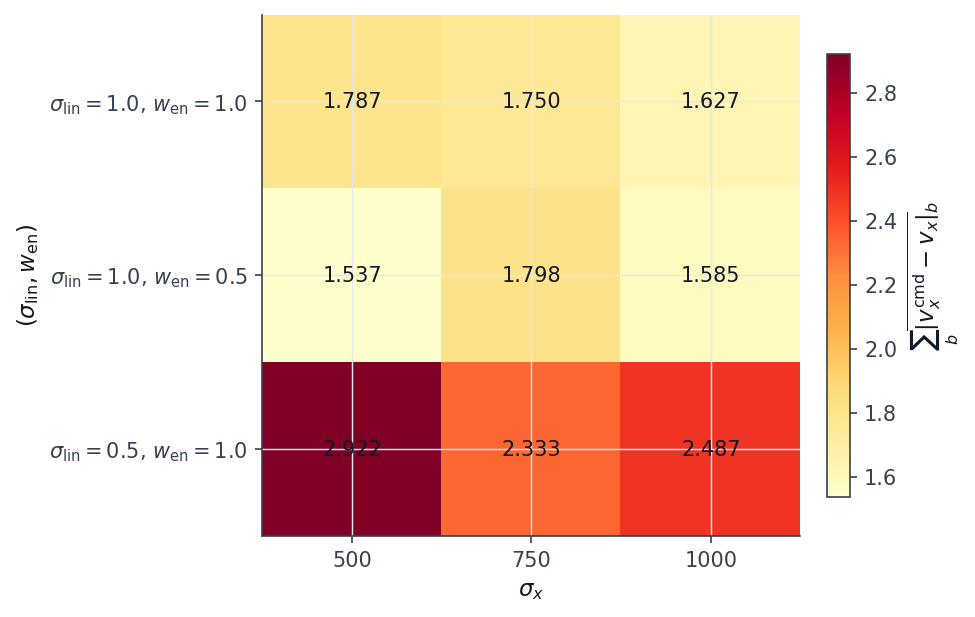
\includegraphics[width=\linewidth]{src/results_phase2_rerun/figures/sigma_phase_v4.png}
\caption{Step 2 calibration grid. Per-bin tracking error (top) and per-bin duty factor (bottom) for each of the nine runs of Table \ref{tab:step2}. Run 7 (selected configuration) is highlighted.}
\label{fig:step2}
\end{figure}

Three observations on Table \ref{tab:step2}. (i) Across all nine cells, no run masters bin 7 ($3.5$--$4.0$ m/s) within the $1500$-iteration grid budget. This is consistent with \S4.1.1, since the grid uses uniform sampling, and uniform alone does not reach the sprint bin even under the energy-regularised reward (cf.\ \S4.3.1). (ii) The $\sigma_v = 0.5$ rows (Runs 1--3) have summed tracking error in the range $2.3$--$2.9$, well above the $\sigma_v = 1.0$ rows ($1.5$--$1.8$). The wider tracking kernel matters more than the choice of $\sigma_{\mathrm{en},x}$ in this grid. (iii) Within the $\sigma_v = 1.0$ rows, the best summed tracking error is Run 7 ($1.537$), and the best gait differential is Run 5 ($0.183$). Run 7 was chosen over Run 5 because the tracking advantage is larger than the gait-differential gap, and because reducing $\alpha_{\mathrm{en}}$ from $1.0$ to $0.5$ leaves more headroom for the curriculum to be the binding constraint on sprint progress (\S4.3).

The chosen tuple is therefore

\[
\sigma_{\mathrm{en},x} = 500, \quad \sigma_{\mathrm{en},z} = 250, \quad \sigma_v = 1.0, \quad \alpha_{\mathrm{en}} = 0.5,
\]

and it is reused unchanged for the matched three-condition sweep of \S4.3.

\subsection{Three Curricula Under the Energy-Regularised Reward}

A second three-condition (uniform, task-specific, teacher-guided) sweep with three independent seeds per condition was run to $3000$ PPO iterations under the energy-regularised reward of \S4.2.1, with the scale parameters fixed at the values chosen by the calibration of \S4.2.2. The remaining experimental configuration (curriculum operators, evaluation protocol, command range, episode length, PPO hyperparameters) is identical to \S4.1, so the two halves of this chapter are directly comparable on a per-cell basis.

\subsubsection{Per-Bin Tracking-Reward Convergence}

Table \ref{tab:phase2_rlin} reports the smoothed per-bin tracking reward $R_j$ at the end of training under the energy-regularised reward, averaged across the three seeds.

\begin{table}[ht]
\centering
\begin{tabularx}{\textwidth}{@{}r r r r r@{}}
\toprule
\textbf{Bin} & $v_x^{\mathrm{cmd}}$ & \textbf{Uniform} & \textbf{Task-specific} & \textbf{Teacher-guided} \\
\midrule
0 & 0.25 m/s & $0.976 \pm 0.001$ & $0.975 \pm 0.001$ & $0.975 \pm 0.002$ \\
1 & 0.75 m/s & $0.971 \pm 0.002$ & $0.970 \pm 0.002$ & $0.970 \pm 0.000$ \\
2 & 1.25 m/s & $0.959 \pm 0.002$ & $0.960 \pm 0.001$ & $0.958 \pm 0.000$ \\
3 & 1.75 m/s & $0.946 \pm 0.001$ & $0.947 \pm 0.001$ & $0.946 \pm 0.001$ \\
4 & 2.25 m/s & $0.934 \pm 0.001$ & $0.935 \pm 0.002$ & $0.936 \pm 0.000$ \\
5 & 2.75 m/s & $0.912 \pm 0.003$ & $0.916 \pm 0.003$ & $0.918 \pm 0.002$ \\
6 & 3.25 m/s & $0.816 \pm 0.002$ & $0.863 \pm 0.016$ & $0.858 \pm 0.006$ \\
7 & 3.75 m/s & $0.001 \pm 0.000$ & $0.703 \pm 0.018$ & $0.693 \pm 0.016$ \\
\bottomrule
\end{tabularx}
\caption{Per-bin tracking reward $R_j$ at end of training, mean $\pm$ std across three seeds, energy-regularised reward of \S4.2.1 with the Run-7 tuple, 3000 PPO iterations per cell. Values are averaged over the last 200 PPO iterations of each run.}
\label{tab:phase2_rlin}
\end{table}

\textbf{What changed from Table \ref{tab:phase1_rlin}.} The plateau on bins 0 through 6 lifts substantially under the energy-regularised reward and the three conditions become indistinguishable there. Every condition reaches $0.97$--$0.98$ at bin 0 and decreases monotonically with the command to $0.82$--$0.86$ at bin 6, with cross-condition gaps below the seed-to-seed noise. The lift is mainly the wider tracking kernel ($\sigma_v = 1.0$ in the Liang reward vs $\sigma_v = 0.5$ in \S3.1.4), which makes $R_{\mathrm{lin}} = \exp(-|\Delta v|^2/\sigma_v)$ saturate near $1$ over a much wider velocity-error window. The bin-monotone decrease is what remains of the same Jensen-type artefact noted in \S4.1.1.

\textbf{Bin 7 is now the only separator.} Task-specific and teacher-guided both clear $\gamma = 0.7$ at bin 7 ($0.70$ and $0.69$ respectively), and uniform collapses to $0.001$. This is the same qualitative collapse uniform had under the sprint-retune reward, but now isolated to the single sprint bin. The energy-regularised reward closes most of the bin-6 gap that uniform had in Phase 1 (uniform reaches $0.82$ at bin 6 here vs $0.06$ in Table \ref{tab:phase1_rlin}) because the cost-of-transport gradient now actively pushes the policy toward a coordinated gait. But at bin 7 even the energy reward is not enough. Uniform's $1/8$ share at the highest command leaves the operator with too few iterations to find a gait that can sustain $3.75$ m/s. Curriculum-driven sampling restores it, and at bin 7 task-specific and teacher-guided are within seed-noise of each other in $R_j$.

\begin{figure}[ht]
\centering
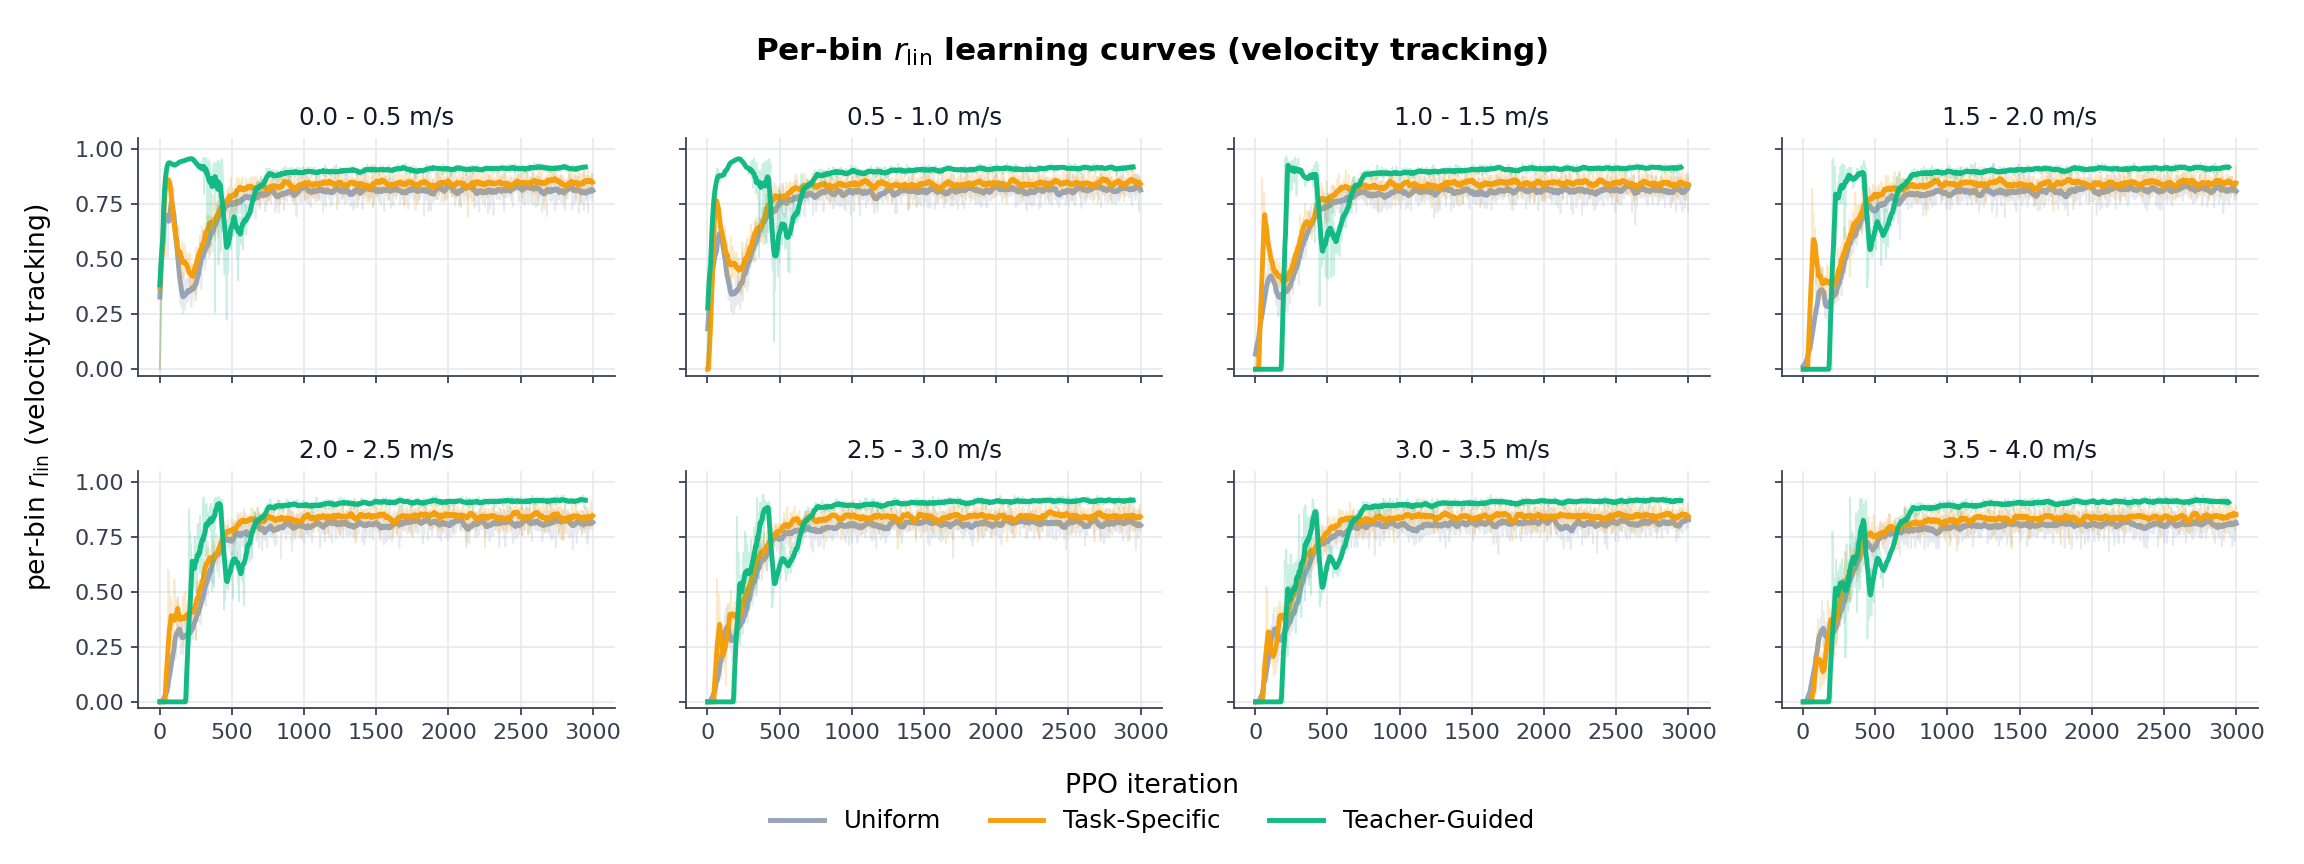
\includegraphics[width=\linewidth]{src/results_phase2_rerun/figures/learning_curves_rlin.png}
\caption{Per-bin tracking-reward curves, energy-regularised reward, three seeds per condition. Rows are velocity bins, columns are curriculum conditions. The mastery threshold $\gamma = 0.7$ is marked as a horizontal reference.}
\label{fig:phase2_lc}
\end{figure}

The iterations-to-mastery metric is summarised in Table \ref{tab:phase2_itm}.

\begin{table}[ht]
\centering
\begin{tabularx}{\textwidth}{@{}r r r r r@{}}
\toprule
\textbf{Bin} & $v_x^{\mathrm{cmd}}$ & \textbf{Uniform} & \textbf{Task-specific} & \textbf{Teacher-guided} \\
\midrule
0 & 0.25 & 24  & 22  & 22 \\
1 & 0.75 & 66  & 98  & 68 \\
2 & 1.25 & 244 & 200 & 268 \\
3 & 1.75 & 294 & 254 & 352 \\
4 & 2.25 & 376 & 312 & 442 \\
5 & 2.75 & 450 & 386 & 558 \\
6 & 3.25 & 614 & 552 & 694 \\
7 & 3.75 & not mastered (0/3) & 1212 (3/3) & 1026 (3/3) \\
\bottomrule
\end{tabularx}
\caption{Iterations-to-mastery per (condition, bin) cell, energy-regularised reward, computed as the first PPO iteration at which the seed-averaged $R_j$ crosses $\gamma = 0.7$. The fraction of seeds that reached mastery individually is shown in parentheses where it is below 3/3.}
\label{tab:phase2_itm}
\end{table}

Bins 0 through 6 are mastered by every condition. Task-specific is fastest on bins 2 through 6 because its monotone-expansion rule concentrates samples on the unlocked edge. Uniform is comparable to teacher-guided through bin 6 and is actually slightly faster than teacher-guided on the upper-middle bins. Under the energy reward the lower bins are easy enough that flat sampling does not lose ground to a learning-progress sampler. At bin 7 the picture inverts. Uniform fails to master at all, while teacher-guided masters first ($1026$) and task-specific masters at $1212$.

\begin{figure}[ht]
\centering
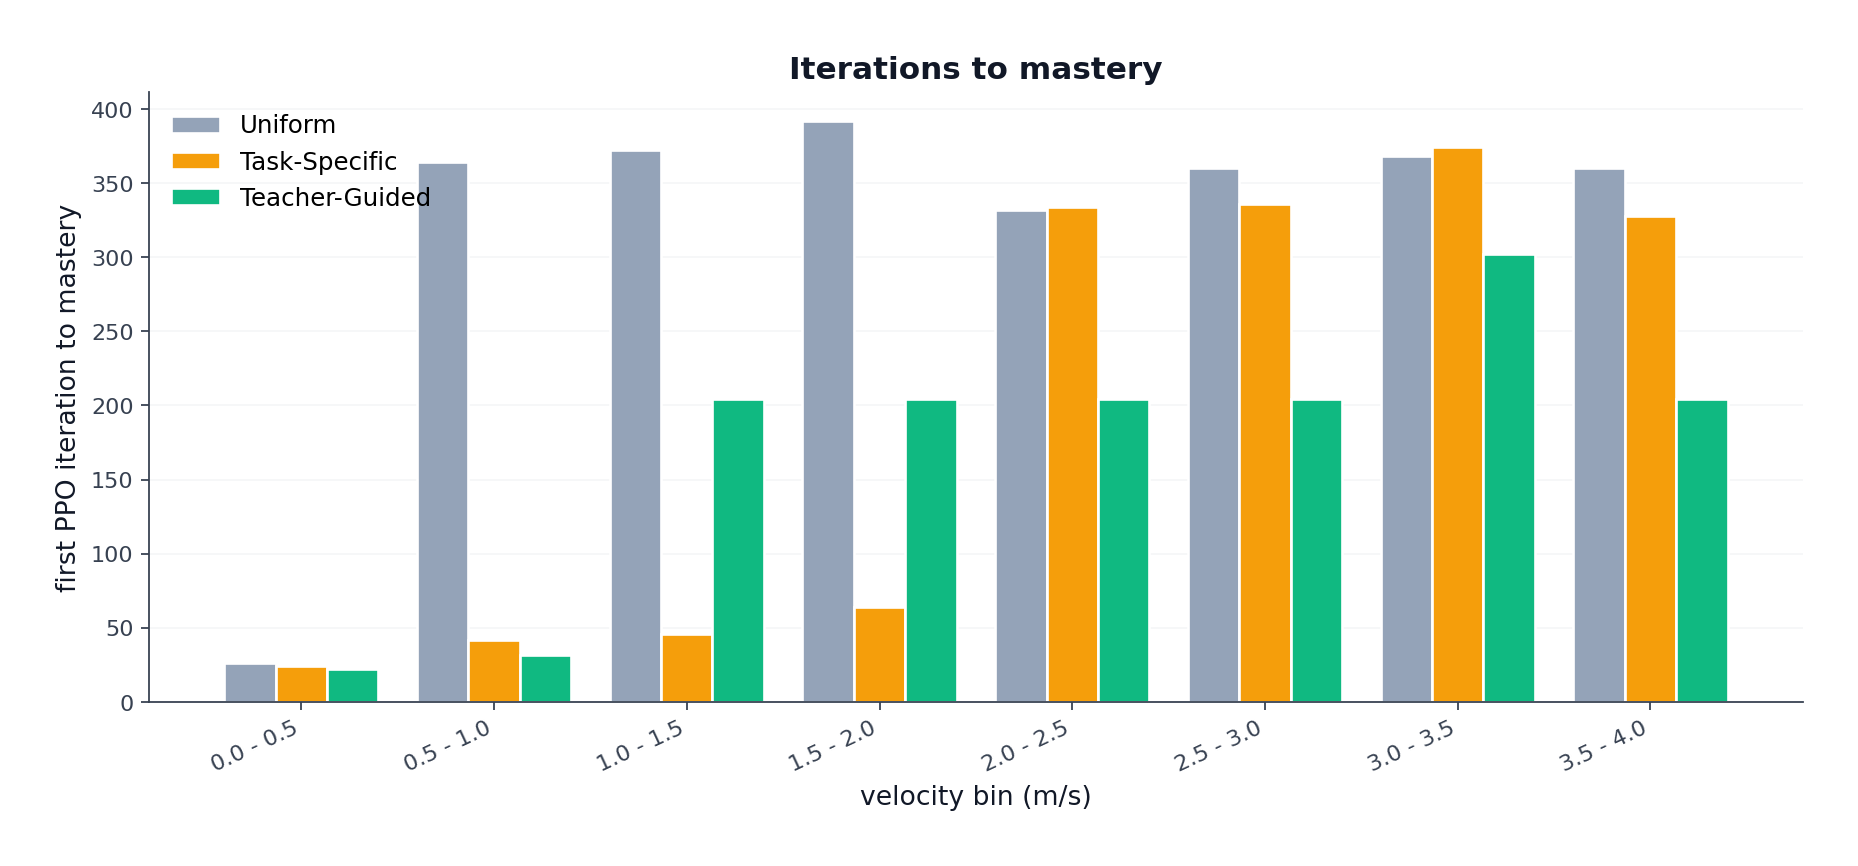
\includegraphics[width=\linewidth]{src/results_phase2_rerun/figures/iterations_to_mastery.png}
\caption{Iterations-to-mastery per (condition, bin), energy-regularised reward. Each bar is the mean across three seeds.}
\label{fig:phase2_itm}
\end{figure}

\begin{figure}[ht]
\centering
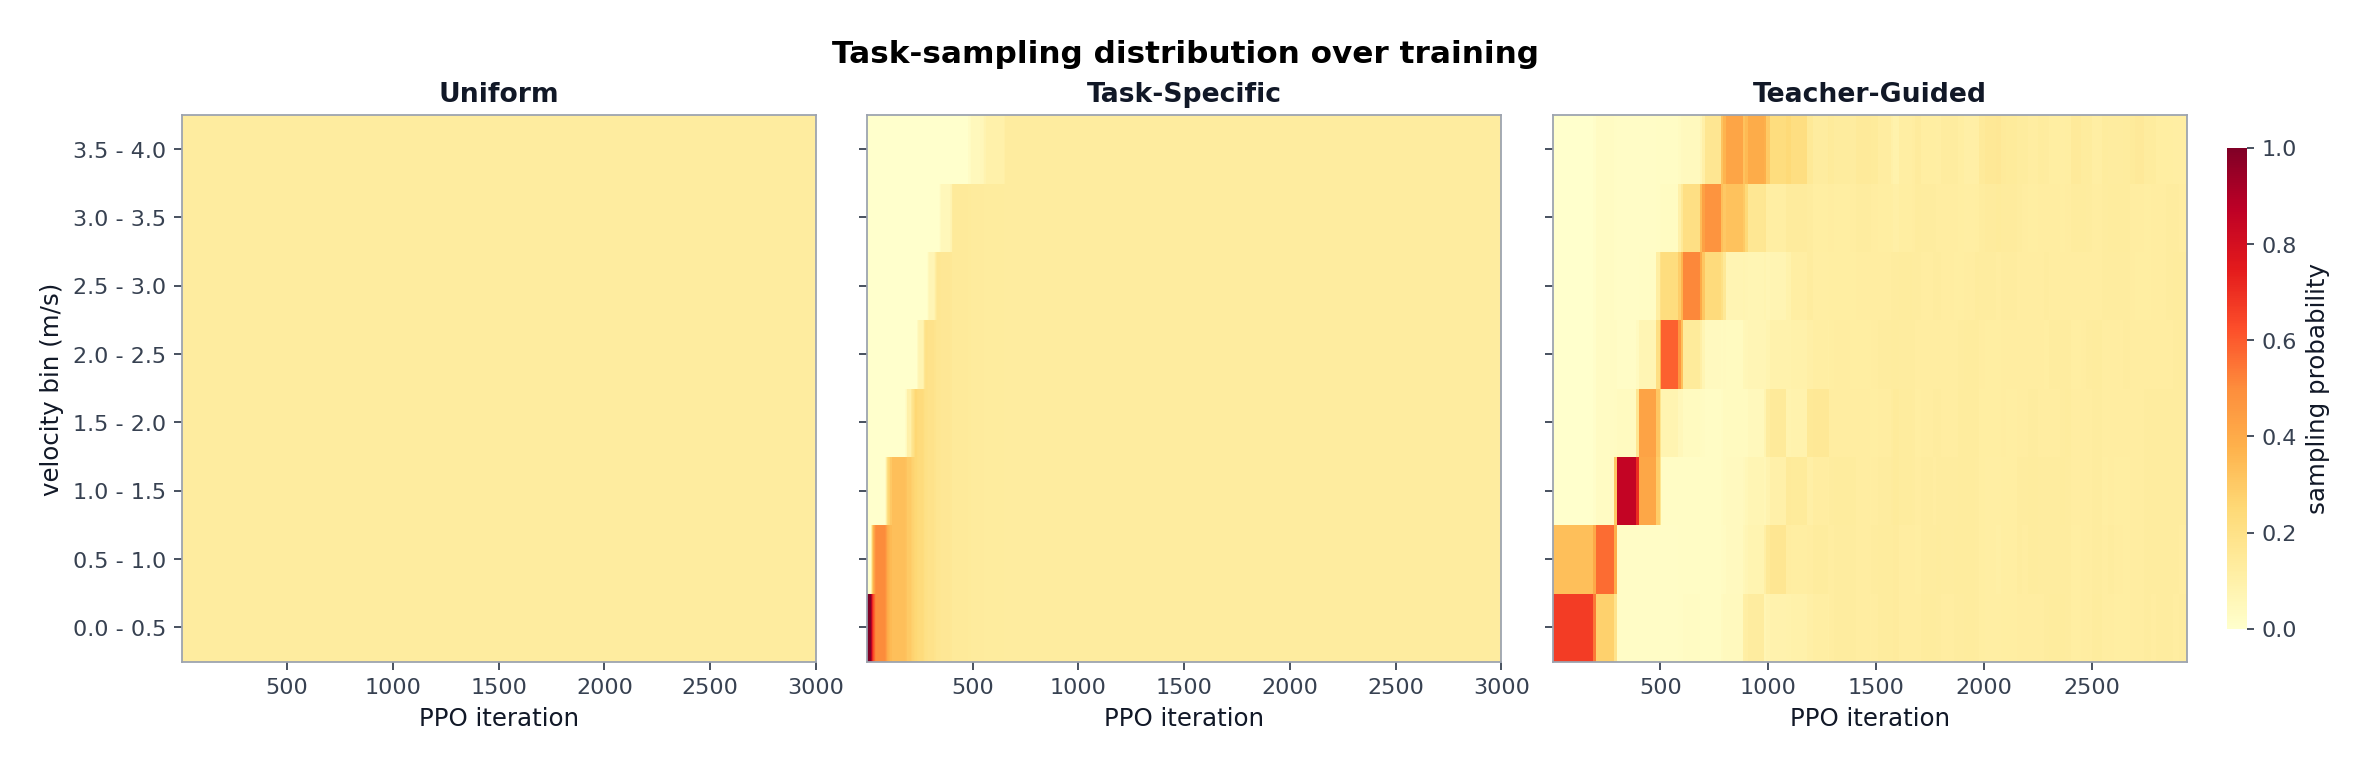
\includegraphics[width=\linewidth]{src/results_phase2_rerun/figures/sampling_heatmap.png}
\caption{Per-bin sampling weight across training, energy-regularised reward. Rows are velocity bins, columns are training iterations. Uniform is flat by construction; task-specific expands its support monotonically; teacher-guided reallocates sampling toward bins with the largest learning progress.}
\label{fig:phase2_heatmap}
\end{figure}

\subsubsection{Per-Bin EPTE-SP}

Table \ref{tab:phase2_epte} reports the EPTE-SP and fall fraction from the deterministic-evaluation protocol of \S3.3, exactly the same metric as Table \ref{tab:phase1_epte} of \S4.1.2 but on the energy-regularised reward.

\begin{table}[ht]
\centering
\begin{tabularx}{\textwidth}{@{}r r r r r@{}}
\toprule
\textbf{Bin} & $v_x^{\mathrm{cmd}}$ & \textbf{Uniform EPTE / fall\%} & \textbf{Task-spec EPTE / fall\%} & \textbf{Teacher EPTE / fall\%} \\
\midrule
0 & 0.25 & $0.432$ / $1\%$ & $0.425$ / $0\%$ & $0.414$ / $2\%$ \\
1 & 0.75 & $0.121$ / $0\%$ & $0.121$ / $0\%$ & $0.122$ / $0\%$ \\
2 & 1.25 & $0.062$ / $0\%$ & $0.061$ / $0\%$ & $0.064$ / $0\%$ \\
3 & 1.75 & $0.054$ / $0\%$ & $0.056$ / $0\%$ & $0.057$ / $0\%$ \\
4 & 2.25 & $0.054$ / $0\%$ & $0.051$ / $0\%$ & $0.056$ / $0\%$ \\
5 & 2.75 & $0.057$ / $0\%$ & $0.055$ / $0\%$ & $0.057$ / $0\%$ \\
6 & 3.25 & $0.092$ / $0\%$ & $0.079$ / $0\%$ & $0.077$ / $0\%$ \\
7 & 3.75 & $0.857$ / $0\%$ & $0.385$ / $0\%$ & $0.126$ / $0\%$ \\
\bottomrule
\end{tabularx}
\caption{Per-bin EPTE-SP and fall fraction, energy-regularised reward, three seeds and 300 rollouts per cell.}
\label{tab:phase2_epte}
\end{table}

Three changes from the Phase 1 row of the same metric (Table \ref{tab:phase1_epte}) are visible. (i) The fall column has collapsed to zero across the board. Under the energy-regularised reward, none of the three conditions falls at any of the eight bins in any meaningful fraction of rollouts. The previously catastrophic bin-6 and bin-7 collapse of uniform, and the $50\%$ fall fraction of task-specific at the sprint bins under \S3.1.4, is gone. (ii) Bins 0 through 6 are within $\sim 10\%$ tracking error for all three conditions (interpreting the $0.4$--$0.5$ EPTE-SP at bin 0 as the normalisation artefact discussed in \S4.1.2). (iii) At bin 7 the three conditions separate sharply. Teacher-guided reaches $0.126$, task-specific reaches $0.385$, and uniform reaches $0.857$.

The bin-7 separation is the central observation of this section. The mean forward velocity at bin 7 under deterministic evaluation is $\bar v_x = 0.54$ m/s for uniform against the $3.75$ m/s command, $\bar v_x = 2.31$ m/s for task-specific, and $\bar v_x = 3.29$ m/s for teacher-guided. Uniform is essentially refusing the sprint command, since the policy walks forward at well below the commanded speed. Task-specific produces a roughly two-thirds-speed walking trot (duty $\beta = 0.59$, no flight phase, see Table \ref{tab:phase2_duty}). Only teacher-guided tracks near the commanded velocity. None of the three falls. The bin-7 EPTE-SP rank is therefore a rank in \textit{what velocity the policy will accept the command at}, not in survival.

\begin{figure}[ht]
\centering
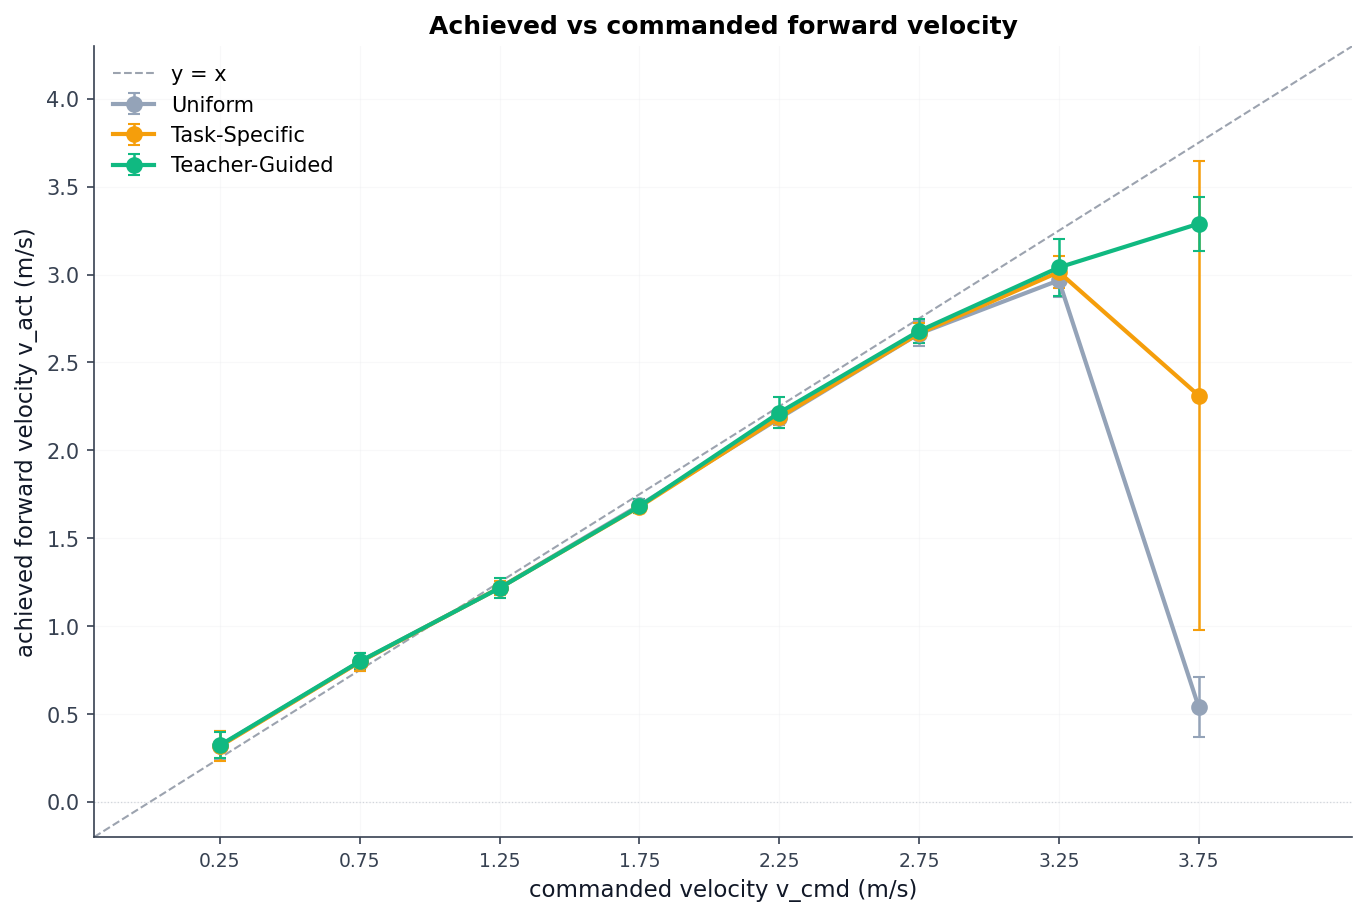
\includegraphics[width=\linewidth]{src/results_phase2_rerun/figures/v_actual_vs_cmd.png}
\caption{Mean measured forward velocity vs commanded velocity, energy-regularised reward. Diagonal is the perfect-tracking reference. Uniform sits near $\bar v_x = 0.5$ m/s at bin 7 against the $3.75$ m/s command; only teacher-guided follows the diagonal through the sprint bin.}
\label{fig:phase2_vvscmd}
\end{figure}

\begin{figure}[ht]
\centering
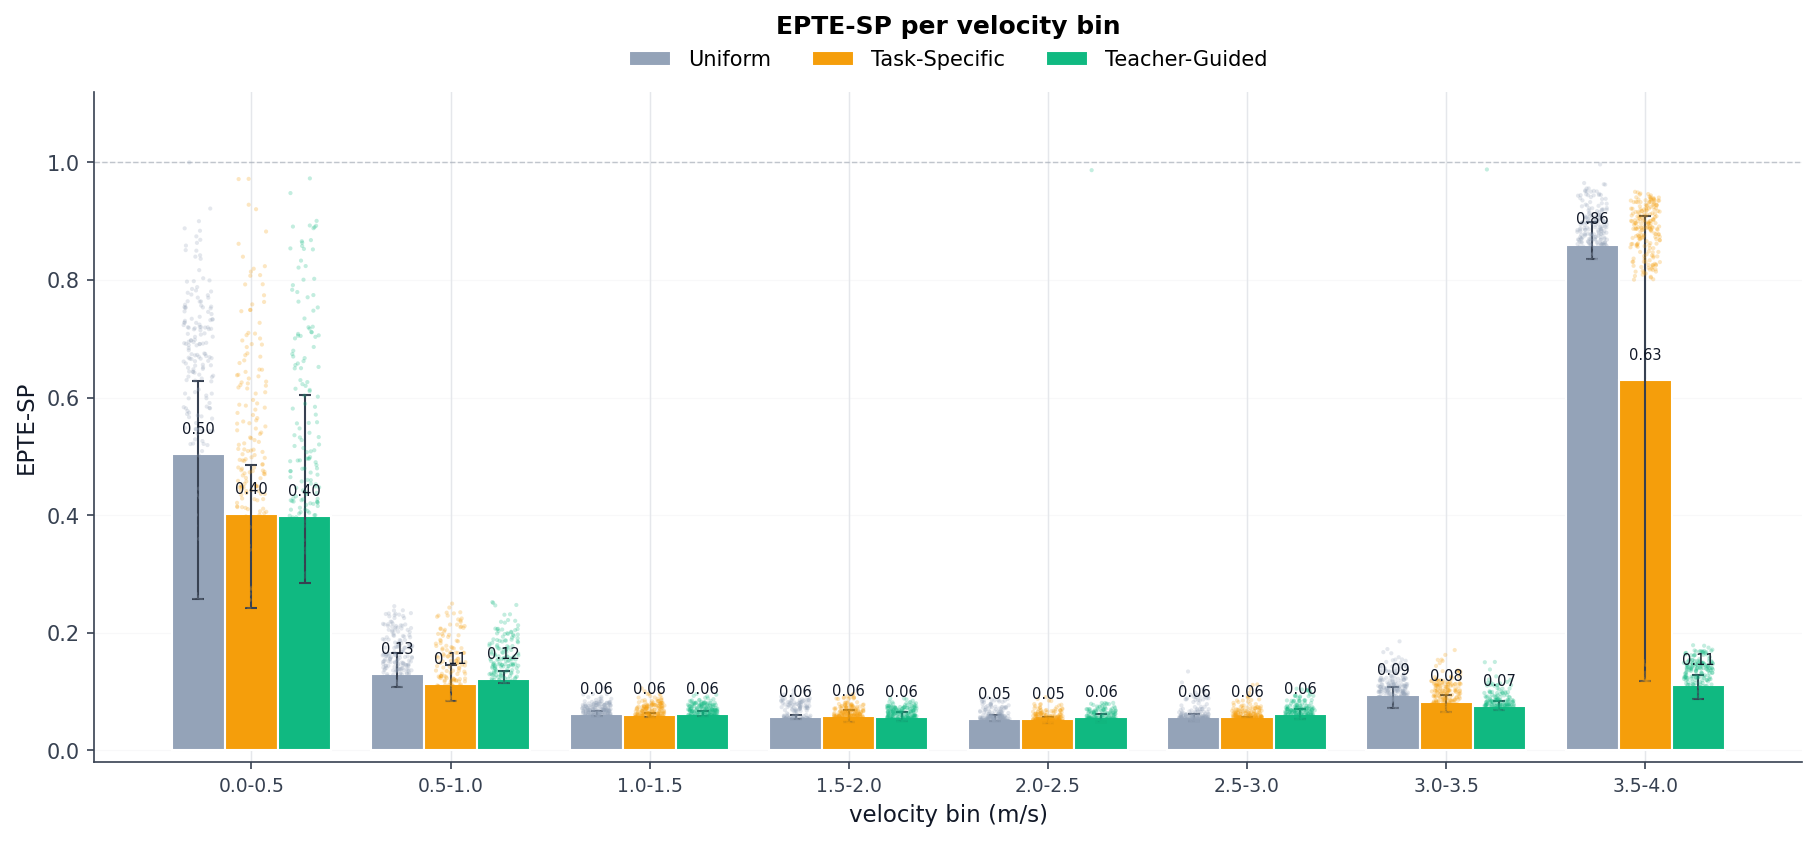
\includegraphics[width=\linewidth]{src/results_phase2_rerun/figures/epte_bars.png}
\caption{EPTE-SP per (condition, bin), energy-regularised reward. Bin-7 bars separate the three conditions: teacher-guided $0.126$, task-specific $0.385$, uniform $0.857$.}
\label{fig:phase2_epte_bars}
\end{figure}

\subsubsection{Qualitative Behaviour at Evaluation}

The low-bin irregular contact pattern of \S4.1.3 is no longer visible under the energy-regularised reward. The irregular four-foot pattern that the \S3.1.4 reward had allowed at slow command is replaced by a coordinated Trot (walking) under all three conditions at bin 0 (Table \ref{tab:phase2_gait}). The sprint-bin collapse that uniform showed at bins 6 and 7 is replaced at bins 0 through 6 by a sustained forward gait. What separates the three conditions at evaluation is the \textit{style} of locomotion at each commanded speed and whether that style matches the speed it is being asked to track at the sprint bin.

\begin{figure}[ht]
\centering
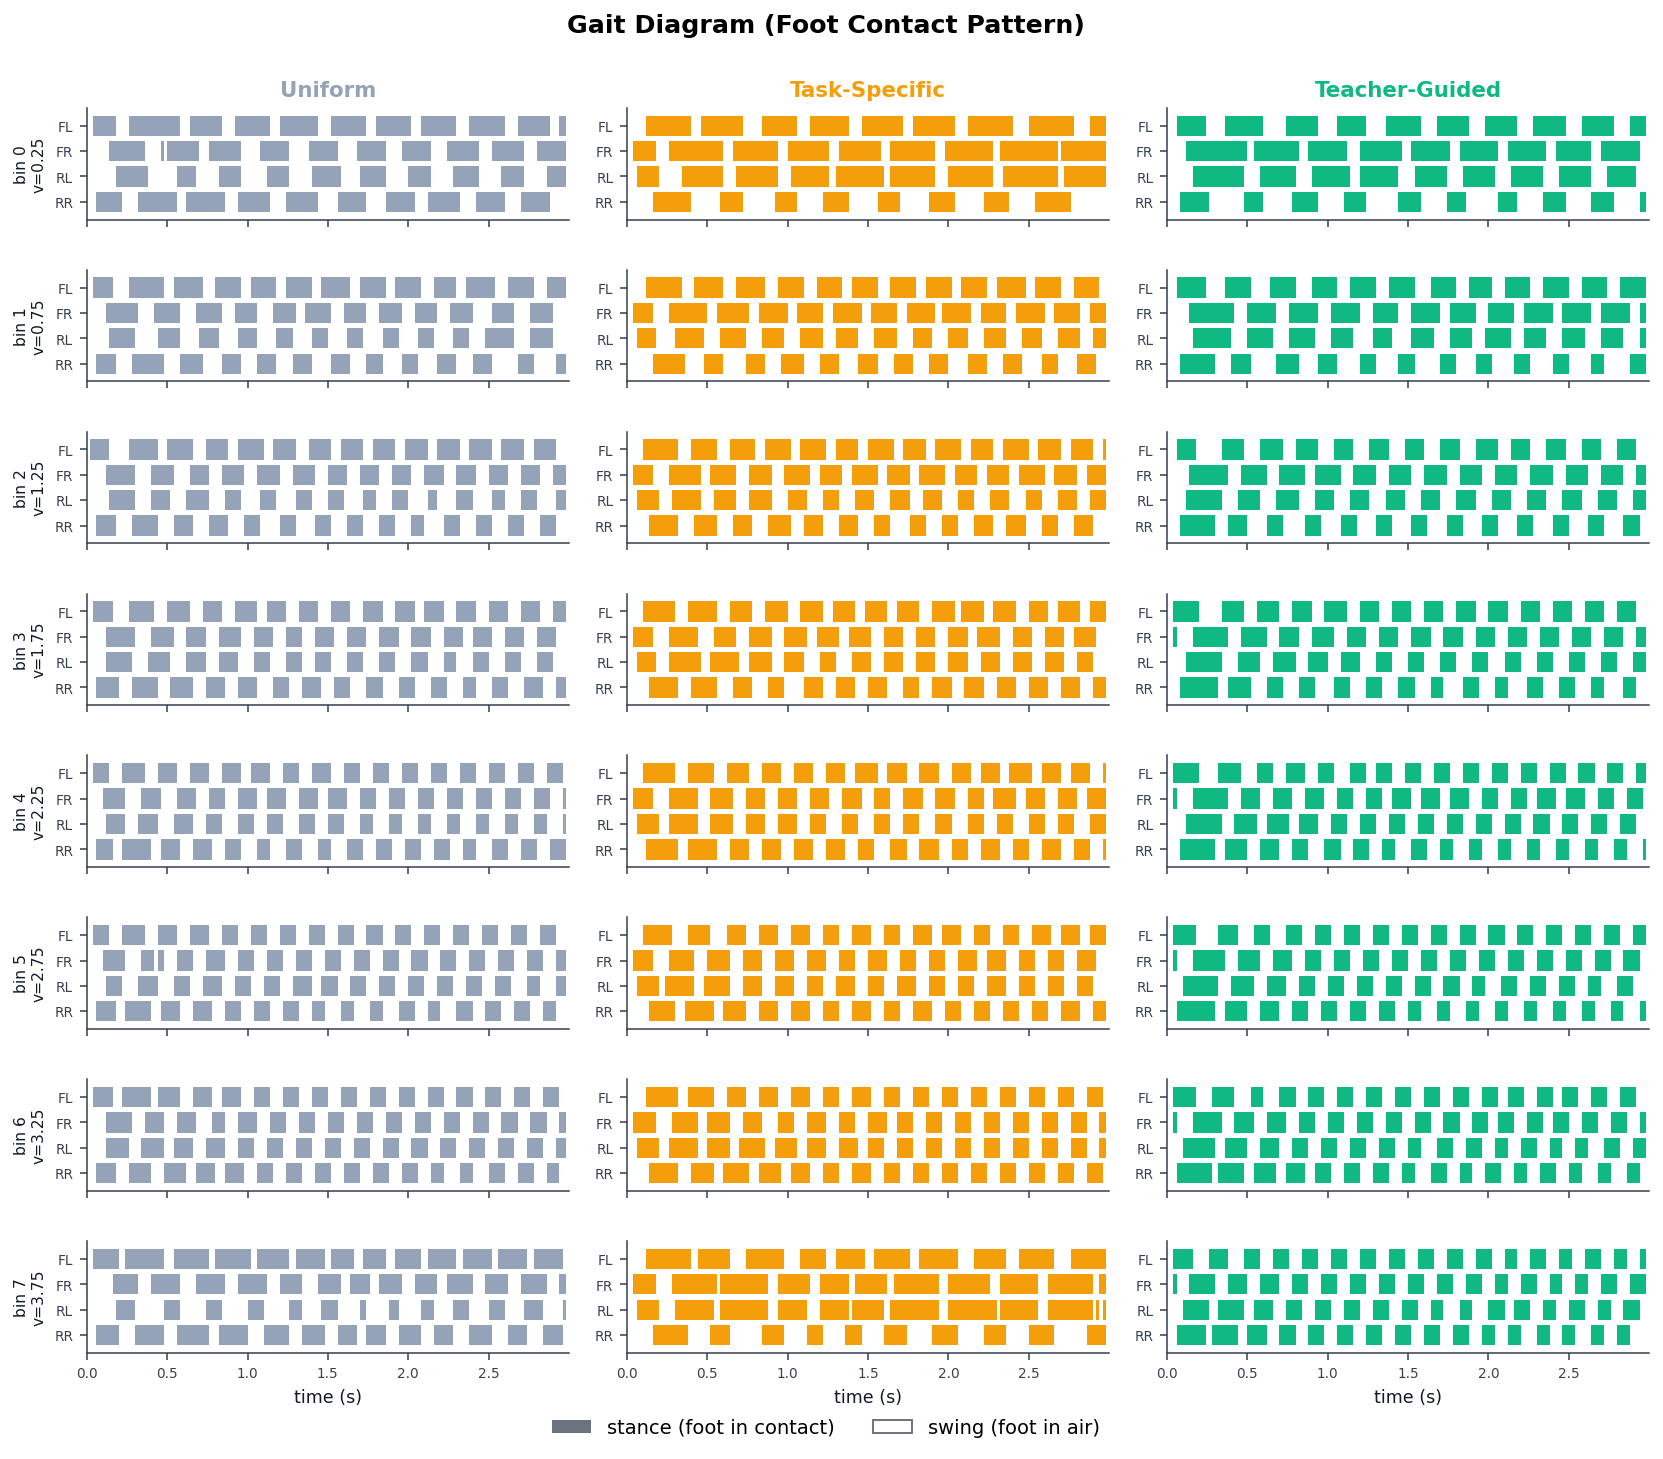
\includegraphics[width=\linewidth]{src/results_phase2_rerun/figures/gait_diagram.png}
\caption{Gait diagram at deterministic evaluation, energy-regularised reward. Columns are conditions (uniform / task-specific / teacher-guided), rows are velocity bins. Coloured blocks mark stance (foot in contact); white gaps mark swing. Per cell the plotted rollout is the best-surviving rollout across the three seeds, with ties broken by closest mean forward velocity to the command.}
\label{fig:phase2_gait}
\end{figure}

\begin{itemize}
  \item \textbf{Uniform.} All eight bins show a clean diagonal-pair Trot pattern, with duty factor $\beta$ declining from $0.67$ at bin 0 to $0.55$ at bins 5--6 (Table \ref{tab:phase2_duty}). At bin 7 stride frequency drops and duty factor rises back to $0.65$, but the diagonal Trot structure is maintained. The policy cannot track the sprint command --- measured velocity is $0.54$ m/s against $3.75$ m/s. Uniform solves survival at the sprint bin (the robot does not fall) but not velocity (it produces a slow Trot instead of sprinting).
  \item \textbf{Task-specific.} Bins 0--1 show a diagonal-pair Trot. From bin 2 the diagonal synchrony weakens and the contact pattern transitions to a four-beat Walk, which holds through bin 4. From bin 5 the pattern shifts to a fore-pair/hind-pair alternation (Bound, walking, $\beta > 0.5$ throughout), which holds through bin 7 ($\beta = 0.59$, $\bar v_x = 2.31$ m/s against the $3.75$ m/s command). This Trot $\to$ Walk $\to$ Bound progression is observed in seed 2 (the best-surviving rollout at the high bins); seeds 0 and 1 show Trot throughout at all bins (\S4.3.4).
  \item \textbf{Teacher-guided.} All eight bins show a clean diagonal-pair Trot throughout. Stride frequency and duty factor scale monotonically with the command from bin 0 ($\beta = 0.67$, $3.4$ Hz) through bin 7 ($\beta = 0.54$, $5.7$ Hz). The diagonal Trot contact pattern is maintained at the sprint bin, and measured velocity at bin 7 is $\bar v_x = 3.29$ m/s against the $3.75$ m/s command. No flight phase occurs in any bin ($\beta > 0.5$ throughout, Table \ref{tab:phase2_duty}).
\end{itemize}

The dominant contact pattern across all three conditions and all eight bins is Trot (walking). Teacher-guided confirms that the energy-regularised reward, \textit{under a curriculum that allocates compute to the harder bins}, maintains a coordinated Trot through the sprint bin. Task-specific (best-surviving seed) shows a Trot $\to$ Walk $\to$ Bound progression at bins 4--7, but this is a single-seed observation within a condition that is otherwise Trot (\S4.3.4). Uniform maintains Trot throughout but cannot achieve sprint velocity: without curriculum-driven sampling at $b_7$, the policy settles in a slow-Trot optimum at the highest command.

\begin{table}[ht]
\centering
\begin{tabularx}{\textwidth}{@{}r r r r r@{}}
\toprule
\textbf{Bin} & $v_x^{\mathrm{cmd}}$ & \textbf{Uniform} $\beta$ / freq & \textbf{Task-spec} $\beta$ / freq & \textbf{Teacher} $\beta$ / freq \\
\midrule
0 & 0.25 m/s & $0.67$ / $3.4$ Hz & $0.66$ / $3.2$ Hz & $0.67$ / $3.4$ Hz \\
1 & 0.75 m/s & $0.60$ / $4.3$ Hz & $0.60$ / $4.4$ Hz & $0.61$ / $4.4$ Hz \\
2 & 1.25 m/s & $0.59$ / $4.7$ Hz & $0.59$ / $4.7$ Hz & $0.59$ / $4.8$ Hz \\
3 & 1.75 m/s & $0.57$ / $5.0$ Hz & $0.58$ / $5.1$ Hz & $0.57$ / $5.1$ Hz \\
4 & 2.25 m/s & $0.56$ / $5.2$ Hz & $0.57$ / $5.5$ Hz & $0.55$ / $5.5$ Hz \\
5 & 2.75 m/s & $0.55$ / $5.4$ Hz & $0.55$ / $5.7$ Hz & $0.54$ / $5.6$ Hz \\
6 & 3.25 m/s & $0.55$ / $5.4$ Hz & $0.55$ / $5.8$ Hz & $0.54$ / $5.7$ Hz \\
7 & 3.75 m/s & $0.65$ / $3.9$ Hz & $0.59$ / $5.3$ Hz & $0.54$ / $5.7$ Hz \\
\bottomrule
\end{tabularx}
\caption{Duty factor and stride frequency per (condition, bin) cell, energy-regularised reward, averaged across three seeds and 300 rollouts per cell. All cells satisfy $\beta > 0.5$ (no flight phase), so the contact patterns are \textit{walking} gaits in the Hildebrand sense.}
\label{tab:phase2_duty}
\end{table}

\subsubsection{Gait Classification}

Gait labels are assigned using two complementary sources: visual inspection of the raw foot-contact diagram (Figure \ref{fig:phase2_gait}), and a per-leg contact correlation analysis computed from the stored rollout traces. The correlation analysis computes the mean Pearson correlation across diagonal leg pairs (FL+RR, FR+RL; high positive $=$ Trot) and across fore/hind pairs (FL+FR, RL+RR; high positive $=$ Bound) for the best-surviving rollout per cell, using the same selection criterion as Figure \ref{fig:phase2_gait}. A cell is labelled \textbf{Trot (walking)} if the diagonal correlation exceeds $+0.5$, \textbf{Bound (walking)} if the fore/hind correlation exceeds $+0.5$, and \textbf{Walk} if both fall below $0.1$. All labels carry $\beta > 0.5$ throughout (Table \ref{tab:phase2_duty}) --- no flight-phase gait occurs in any cell. The three labels are:

\begin{table}[ht]
\centering
\begin{tabularx}{\textwidth}{@{}X c X r@{}}
\toprule
\textbf{Label} & $\beta$ & \textbf{Footfall pattern} & \textbf{Speed} \\
\midrule
Walk & $> 0.5$ & Four-beat, each foot offset by $\approx \tfrac{1}{4}$ stride & Slowest \\
\addlinespace
Trot (walking) & $> 0.5$ & Diagonal pairs (FL+RR, FR+RL) alternating, no flight phase & Medium \\
\addlinespace
Bound (walking) & $> 0.5$ & Fore pair (FL+FR) and hind pair (RL+RR) alternating, no flight phase & Faster \\
\bottomrule
\end{tabularx}
\caption{Gait labels used in the Phase 2 sweep. All observed labels have $\beta > 0.5$, confirming no flight-phase gaits occurred.}
\label{tab:gait_labels}
\end{table}

Per (condition, bin) cell, the label is taken from the best-surviving rollout using the same criterion as Figure \ref{fig:phase2_gait}. For task-specific, two seeds (seeds 0 and 1) show Trot throughout at all bins; the pattern below reflects seed 2, which is the best-surviving rollout at high-speed bins and shows a different progression (marked $\dagger$):

\begin{table}[ht]
\centering
\begin{tabularx}{\textwidth}{@{}r r X X X@{}}
\toprule
\textbf{Bin} & $v_x^{\mathrm{cmd}}$ & \textbf{Uniform} & \textbf{Task-specific} & \textbf{Teacher-guided} \\
\midrule
0 & 0.25 m/s & Trot (walking) & Trot (walking)           & Trot (walking) \\
1 & 0.75 m/s & Trot (walking) & Trot (walking)           & Trot (walking) \\
2 & 1.25 m/s & Trot (walking) & Walk$^\dagger$            & Trot (walking) \\
3 & 1.75 m/s & Trot (walking) & Walk$^\dagger$            & Trot (walking) \\
4 & 2.25 m/s & Trot (walking) & Walk$^\dagger$            & Trot (walking) \\
5 & 2.75 m/s & Trot (walking) & Bound (walking)$^\dagger$ & Trot (walking) \\
6 & 3.25 m/s & Trot (walking) & Bound (walking)$^\dagger$ & Trot (walking) \\
7 & 3.75 m/s & Trot (walking) & Bound (walking)$^\dagger$ & Trot (walking) \\
\bottomrule
\end{tabularx}
\caption{Gait label per (condition, bin) cell at deterministic evaluation, energy-regularised reward, from the best-surviving rollout per cell (matching Figure \ref{fig:phase2_gait} selection). Labels confirmed by per-leg contact correlation (\S4.3.4). $^\dagger$Single-seed observation (seed 2 only); seeds 0 and 1 for task-specific show Trot (walking) at all bins.}
\label{tab:phase2_gait}
\end{table}

Three features of Table \ref{tab:phase2_gait} are notable.

\textbf{Teacher-guided: Trot throughout.} The diagonal-pair contact pattern holds across all eight bins. Stride frequency and duty factor continue scaling with the command through bin 7 ($\beta = 0.54$, $5.7$ Hz), and measured velocity is $3.29$ m/s against the $3.75$ m/s command. Teacher-guided is the only condition that holds the Trot pattern with sprint-speed tracking.

\textbf{Task-specific: Trot $\to$ Walk $\to$ Bound (single-seed observation).} The best-surviving rollout (seed 2) shows Trot at bins 0--1, a four-beat Walk from bins 2--4 (diagonal correlation weakens to $+0.09$--$+0.40$, below the Trot threshold), and fore-pair/hind-pair alternation from bin 5 onward (Bound, walking, $\beta > 0.5$), reaching $\bar v_x = 2.31$ m/s against the $3.75$ m/s command at bin 7. Seeds 0 and 1 show Trot throughout at all bins. The Walk and Bound labels at bins 2--7 are a within-condition, single-seed observation rather than a condition-level finding.

\textbf{Uniform: Trot throughout but speed-limited.} The diagonal-pair pattern is visible across all bins. At bin 7 stride frequency drops and duty factor rises to $0.65$, yet the Trot footfall structure is maintained. The policy cannot track the sprint command --- measured velocity is only $0.54$ m/s against $3.75$ m/s. Uniform produces the Trot contact pattern but not sprint velocity.

Under a fixed energy-regularised reward and fixed budget, the dominant contact pattern is Trot (walking) across all three conditions. Teacher-guided maintains Trot with sprint-speed tracking. Task-specific (in the best-seed rollout) shows Trot $\to$ Walk $\to$ Bound at bins 2--7, but the other two seeds show Trot throughout; the Bound observation is a within-condition seed-level variant. Uniform maintains Trot but cannot achieve sprint velocity. A curriculum that allocates non-trivial compute to the highest bin is required for sprint-speed tracking, regardless of which contact pattern it produces.
